\documentclass[
	% -- opções da classe memoir --
	12pt,				% tamanho da fonte
	%openright,			% capítulos começam em pág ímpar (insere página vazia caso preciso)
	oneside,			% para impressão no anverso. Oposto a twoside
	a4paper,			% tamanho do papel. 
	% -- opções da classe abntex2 --
	chapter=TITLE,		% títulos de capítulos convertidos em letras maiúsculas
	section=TITLE,		% títulos de seções convertidos em letras maiúsculas
	%subsection=TITLE,	% títulos de subseções convertidos em letras maiúsculas
	%subsubsection=TITLE,% títulos de subsubseções convertidos em letras maiúsculas
	% -- opções do pacote babel --
	english,
	brazil
	]{abntex2}

\usepackage{setup/ufscthesisA4-alf}
\usepackage{setup/my_styles}

% ---
% Filtering and Mapping Bibliographies
% ---
% Pacotes de citações
% ---
\usepackage{csquotes}
\usepackage[backend = biber, style = abnt]{biblatex}
% FIXME Se desejar estilo numérico de citações,  comente a linha acima e descomente a linha a seguir.
% \usepackage[backend = biber, style = numeric-comp]{biblatex}

\setlength\bibitemsep{\baselineskip}
\DeclareFieldFormat{url}{Disponível~em:\addspace\url{#1}}
\NewBibliographyString{sineloco}
\NewBibliographyString{sinenomine}
\DefineBibliographyStrings{brazil}{%
	sineloco     = {\mkbibemph{S\adddot l\adddot}},
	sinenomine   = {\mkbibemph{s\adddot n\adddot}},
	andothers    = {\mkbibemph{et\addabbrvspace al\adddot}},
	in			 = {\mkbibemph{In:}}
}

\addbibresource{references.bib} % Seus arquivos de referências

% ---
\DeclareSourcemap{
	\maps[datatype=bibtex]{
		% remove fields that are always useless
		\map{
			\step[fieldset=abstract, null]
			\step[fieldset=pagetotal, null]
		}
		% remove URLs for types that are primarily printed
%		\map{
%			\pernottype{software}
%			\pernottype{online}
%			\pernottype{report}
%			\pernottype{techreport}
%			\pernottype{standard}
%			\pernottype{manual}
%			\pernottype{misc}
%			\step[fieldset=url, null]
%			\step[fieldset=urldate, null]
%		}
		\map{
			\pertype{inproceedings}
			% remove mostly redundant conference information
			\step[fieldset=venue, null]
			\step[fieldset=eventdate, null]
			\step[fieldset=eventtitle, null]
			% do not show ISBN for proceedings
			\step[fieldset=isbn, null]
			% Citavi bug
			\step[fieldset=volume, null]
		}
	}
}

% ---
% Informações de dados para CAPA e FOLHA DE ROSTO
% ---
\autor{Patrick Hoeckler}
\titulo{An Analysis of Techniques for Building Generative Adversarial Networks}
%\subtitulo{Subtítulo (se houver)}
\orientador{Prof. Fabrício de Oliveira Ourique, Dr.}
% Coordenador do curso.
\coordenador{Prof. Fabrício de Oliveira Ourique, Dr.}
% Ano em que o trabalho foi defendido.
\ano{2021}
% Data em que ocorreu a defesa.
\data{03 de Maio de 2021}
% Cidade em que ocorreu a defesa.
\local{Araranguá}
\instituicaosigla{UFSC}
\instituicao{Universidade Federal de Santa Catarina}
\tipotrabalho{Trabalho de Conclusão de Curso}
\formacao{Bacharel em Engenharia de Computação}
\nivel{Bacharel}
\programa{Curso de Graduação em Engenharia de Computação}
\centro{Centro de Ciências, Tecnologias e Saúde do Campus Araranguá}

\preambulo {
    \imprimirtipotrabalho~do~\imprimirprograma~do~\imprimircentro~da~\imprimirinstituicao~para~a~obtenção~do~título~de~\imprimirformacao.
}

% ---
% Configurações de aparência do PDF final
% ---
% alterando o aspecto da cor azul
\definecolor{blue}{RGB}{41,5,195}
% informações do PDF
\makeatletter
\hypersetup{
     	%pagebackref=true,
		pdftitle={\@title}, 
		pdfauthor={\@author},
    	pdfsubject={\imprimirpreambulo},
	    pdfcreator={LaTeX with abnTeX2},
		pdfkeywords={ufsc, latex, abntex2}, 
		colorlinks=true,       		% false: boxed links; true: colored links
    	linkcolor=black,%blue,          	% color of internal links
    	citecolor=black,%blue,        		% color of links to bibliography
    	filecolor=black,%magenta,      		% color of file links
		urlcolor=black,%blue,
		bookmarksdepth=4
}
\makeatother
% ---

\siglalista{MNIST}{Modified National Institute of Standards and Technology database}
\siglalista{CIFAR}{Canadian Institute for Advanced Research}

\siglalista{KNN}{K-Nearest Neighbours}
\siglalista{SVM}{Support Vector Machine}
\siglalista{CNN}{Convolutional Neural Network}
\siglalista{FC}{Fully Connected}

\siglalista{DL}{Deep Learning}
\siglalista{MLP}{Multilayer Perceptron}
\siglalista{LSTM}{Long Short-Term Memory}
\siglalista{RNN}{Recurrent Neural Network}
\siglalista{ResNet}{Residual Networks}
\siglalista{MSE}{Mean Squared Error}

\siglalista{GAN}{Generative Adversarial Network}
\siglalista{DCGAN}{Deep Convolutional GAN}
\siglalista{CGAN}{Conditional GAN}
\siglalista{WGAN}{Wassertein GAN}
\siglalista{WGAN-GP}{WGAN with Gradient Penalization}

\siglalista{EM}{Earth-Mover}

\siglalista{ReLU}{Rectified Linear Unit}
\siglalista{tanh}{hyperbolic tangent}

\siglalista{SGD}{Stochastic Gradient Descent}
\siglalista{Adam}{Adaptive Moment Estimation}

\siglalista{FID}{Fréchet Inception Distance}
\siglalista{FCD}{Fréchet Classifier Distance}
\siglalista{IS}{Inception Score}
\siglalista{CS}{Classifier Score}

\siglalista{BS}{Batch Size}
\siglalista{BN}{Batch Normalization}
\siglalista{UP}{Upscaling Method}
\siglalista{OPT}{Optimizer}
\siglalista{LDIM}{Dimensions of latent space}
\siglalista{CLIP}{Clipping value for the parameters of the critic}
\siglalista{NCRIT}{Number of updates to critic before update to generator}
\siglalista{SMOOTH}{Value of one-sided label smoothing}
\simbololista{sigmoid}{\ensuremath{\sigma}}{Sigmoid function}
\simbololista{theta}{\ensuremath{\theta}}{Trainable Parameters of the Neural Network}
\simbololista{lambda}{\ensuremath{\lambda}}{Regularization strength}
\simbololista{epsilon}{\ensuremath{\epsilon}}{Computational stability term}
\simbololista{latent_space}{\ensuremath{\mathcal{Z}}}{Latent space of the generator}
\simbololista{input_space}{\ensuremath{\mathcal{X}}}{Input space}
\simbololista{expected_value}{\ensuremath{\mathbb{E}}}{Expected value}

\simbololista{learning_rate}{\ensuremath{\eta}}{Learning Rate}
\simbololista{beta_1}{\ensuremath{\beta_1}}{Momentum hyperparameter of Adam}

% compila a lista de abreviaturas e siglas e a lista de símbolos
\makenoidxglossaries

% compila o indice
\makeindex

\begin{document}

\selectlanguage{english}  % Seleciona o idioma do documento (conforme pacotes do babel)
\frenchspacing  % Retira espaço extra obsoleto entre as frases.
\OnehalfSpacing  % Espaçamento 1.5 entre linhas

% Corrige justificação
%\sloppy

% ELEMENTOS PRÉ-TEXTUAIS
% ---
% Capa
% ---
\imprimircapa
% ---

% ---
% Folha de rosto
% (o * indica que haverá a ficha bibliográfica)
% ---
\imprimirfolhaderosto*
% ---

% ---
% Inserir a ficha bibliografica
% ---
% http://ficha.bu.ufsc.br/
\begin{fichacatalografica}
	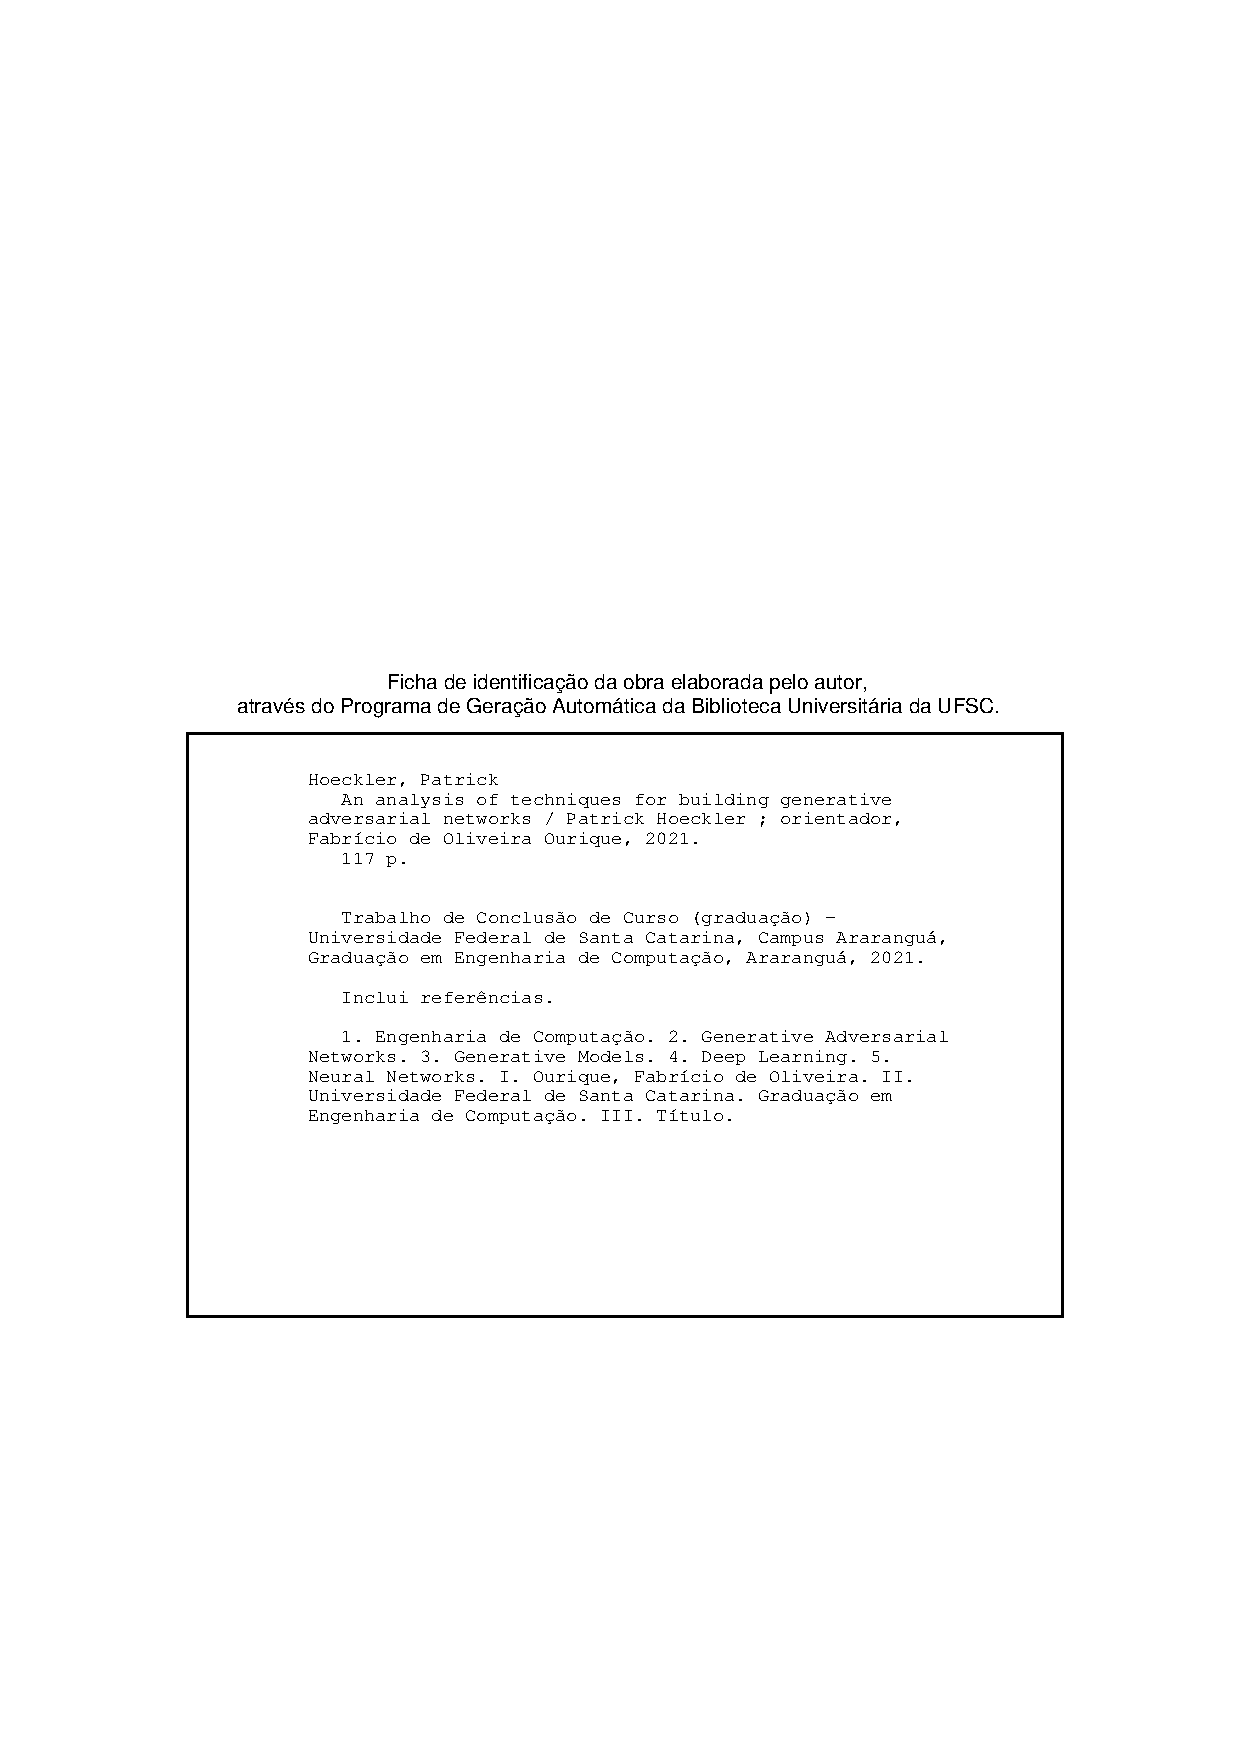
\includepdf{beforetext/Ficha_Catalografica.pdf}
\end{fichacatalografica}
% ---

% ---
% Inserir folha de aprovação
% ---
\begin{folhadeaprovacao}
	\OnehalfSpacing
	\centering
	\imprimirautor\\%
	\vspace*{10pt}		
	\textbf{\imprimirtitulo}%
	\ifnotempty{\imprimirsubtitulo}{:~\imprimirsubtitulo}\\%
	%		\vspace*{31.5pt}%3\baselineskip
	\vspace*{\baselineskip}
	%\begin{minipage}{\textwidth}
	% ~do~\imprimirprograma~do~\imprimircentro~da~\imprimirinstituicao~para~a~obtenção~do~título~de~\imprimirformacao.
	Este~\imprimirtipotrabalho~foi julgado adequado para obtenção do Título de \imprimirformacao ~e aprovado em sua forma final pelo~\imprimirprograma. \\
		\vspace*{\baselineskip}
	\imprimirlocal, \imprimirdata. \\
	\vspace*{2\baselineskip}
	\assinatura{\OnehalfSpacing\imprimircoordenador \\ \imprimircoordenadorRotulo~do Curso}
	\vspace*{2\baselineskip}
	\textbf{Banca Examinadora:} \\
	\vspace*{\baselineskip}
	\assinatura{\OnehalfSpacing\imprimirorientador \\ Orientador}
	%\end{minipage}%
	\vspace*{\baselineskip}
	\assinatura {
	    Prof. Antônio Carlos Sobieranski, Dr.\\
	    Avaliador \\
	    Universidade Federal de Santa Catarina
    }

	\vspace*{\baselineskip}
	\assinatura {
    	Prof. Alexandre Leopoldo Gonçalves, Dr.\\
    	Avaliador \\
    	Universidade Federal de Santa Catarina
	}


\end{folhadeaprovacao}
% ---

\begin{dedicatoria}
	\vspace*{\fill}
	\noindent
	\begin{adjustwidth*}{}{6.5cm}     
		For CEP
	\end{adjustwidth*}
\end{dedicatoria}
\begin{agradecimentos}
Eu gostaria muito que essa parte estivesse em branco, que eu pudesse dizer que fiz tudo sozinho e não tive nenhuma ajuda, mas não foi bem assim que aconteceu, eu não teria chegado até aqui se eu tivesse vindo sozinho. Tem algumas pessoas que eu gostaria de agradecer.

Mantendo o clichê, eu primeiro tenho que agradecer a minha mãe. Ela não teve muita influência direta nessa minha formação, eu até estava me questionando se fazia sentido incluir ela aqui já que não parecia que ela teve muito a ver com essa parte da minha vida. Mas aí eu percebi que eu estava sendo maluco, eu não consigo pensar em nenhuma pessoa que tenha feito mais por mim do que minha mãe, se olhar para as influências indiretas vai dar de perceber claramente que elas são bem maiores do que qualquer influência que os outros possam ter tido.

Eu tenho quase certeza de que se tirassem qualquer outra pessoa da minha vida eu ainda teria conseguido chegar aqui, seria bem mais sofrido, mas eu teria chegado. Mas se tirasse a minha mãe eu nem sei se eu teria conseguido começar a faculdade. O clichê é clichê por um motivo, obrigado mãe.

Mas partindo pra influências mais diretas, meu pai, fazer a faculdade sem a ajuda que meu pai me deu teria sido muito mais sofrido. Ele foi quem me manteve alimentado e com um teto em cima da cabeça, eu não sei como eu teria feito sem tua ajuda pai.

Seguindo o baile para os meus colegas de apartamento, Gustavo (o Gino) e Caio. O Gino foi quem me apresentou esse curso e dividiu o apartamento comigo durante todo o curso, o Caio entro lá pelo meio do tempo pra trazer mais alegria e principalmente pra baratear mais o aluguel, sempre é bom. Bons tempos, boas lembraças, algumas não tão boas, mas ainda estamos no lucro.

A meus bons amigos que fiz no curso, em especial o Ramom, o Ricardo e o Felipe, grandes camaradas. Também tive o prazer de trabalhar com alguns professores aqui da UFSC que me fizeram aprender muita coisa e conseguir uma renda extra (sempre é bom), em especial gostaria de agradecer ao professor Marcelo Zannin da Rosa, ótima pessoa e com um ótimo gosto para camisetas. Espero que a bondade que vocês mostraram para mim possa voltar para vocês.

Também gostaria de agradecer meus avaliadores Alexandre L. Gonçalves e Antônio C. Sobieranski junto com meu orientador Fabrício de Oliveira Ourique, minhas aulas com vocês estão entre as melhores e as quais eu aprendi mais. O Fabrício também foi um ótimo orientador, além de me ajudar com o TCC me ajudou com várias dúvidas que eu tinha sobre o estágio.

Por último eu gostaria de agradecer a todos aqueles que estão lutando pela educação gratuita, com certeza essas pessoas tiveram um enorme impacto em tudo o que eu aprendi aqui na faculdade. Tudo o que eu fiz nesse TCC eu aprendi gratuitamente, eu acho incrível que eu possa sentar na minha casa e assistir cursos completos do MIT, de Harvard, de Stanford e todos os outros. Eu não teria aprendido tanto se não fosse por todas essas pessoas e eu torço que isso consiga chegar pra todo mundo um dia.

\end{agradecimentos}
% \include{beforetext/epigrafe}
\setlength{\absparsep}{18pt} % ajusta o espaçamento dos parágrafos do resumo

\begin{resumo}
	\SingleSpacing
	Generative Adversarial Networks (GANs) are a subcategory of Artificial Neural Networks where the objective is the generation of new data, they do that by modeling the probability distribution of real data, usually coming from a dataset, and sampling from the modeled distribution in order to produce original data that is similar, and optimally indistinguishable, from what was used in training.
	The principle behind GANs is based on a competition between two different networks, a discriminator who tries to distinguish real from fake data, and a generator who tries to fool the discriminator by producing data that is as close to the real one as possible.
	However, the competition between the networks makes training GANs be something notoriously difficult, instability and non-convergence are a common occurrence and many techniques have been proposed to improve not only the learning process, but also the quality of the generated results.
	The goal for this document was to analyse a number of the most common approaches and make an empirical evaluation of those, trying to apply the techniques in different datasets and seeing which configuration produces the best results. In the end there should be a roadmap that can be used to help guide the initial decisions about what method to use when constructing GANs for new and unknown situations.
	
	\textbf{Keywords}: Deep Learning. Neural Networks. Generative models. Generative Adversarial Networks. GAN.
\end{resumo}



\begin{resumo}[Resumo]
	\SingleSpacing
	\begin{otherlanguage*}{brazil}
		Generative Adversarial Networks (GANs) são uma subcategoria de Rede Neurais Artificiais onde o objetivo é a geração de novos dados, elas fazem isso tentando modelar a distribuição de probabilidades de dados reais, geralmente vindos de um dataset, e amostrando da distribuição modelada de modo a produzir dados originais que são similares, e idealmente indistinguíveis do que foi usado durante o treino.
    	O princípio por trás de GANs é baseado em uma competição entre duas redes distintas, um discriminador que tenta distinguir entre dados reais e falsos, e um gerador que tenta enganar o discriminador produzindo dados que são o mais perto possível dos dados reais.
    	Entretanto, a competição entre as duas redes faz do treinamento de GANs algo que é notoriamente difícil, instabilidade e não-convergência são ocorrências comuns e muitas técnicas foram propostas para melhorar não apenas o processo de aprendizado, mas também a qualidade dos resultados gerados.
    	O objetivo deste documento foi de analisar um número de abordagens mais comuns e realizar uma avaliação empírica destas, tentando aplicar as técnicas em diferentes datasets e observando qual configuração produz os melhores resultados. Ao fim deve haver um roteiro que pode ser usado para ajudar a guiar as decisões iniciais sobre qual método utilizar ao construir GANs para novas situações desconhecidas.
    	
    	\textbf{Palavras-chave}: Deep Learning. Neural Networks. Modelos generativos. Generative Adversarial Networks. GAN.
	\end{otherlanguage*}
\end{resumo}


{ %hidelinks
	\hypersetup{hidelinks}
	% inserir lista de ilustrações
	\pdfbookmark[0]{\listfigurename}{lof}
	\listoffigures*
	\cleardoublepage
	
	% inserir lista de quadros
    % 	\pdfbookmark[0]{\listofquadrosname}{loq}
    % 	\listofquadros*
    % 	\cleardoublepage
	
	% inserir lista de tabelas
% 	\pdfbookmark[0]{\listtablename}{lot}
% 	\listoftables*
% 	\cleardoublepage
	
	% inserir lista de siglas e lista de simbolos
	\imprimirlistadesiglas
	\imprimirlistadesimbolos
	
	% inserir o sumario
	\pdfbookmark[0]{\contentsname}{toc}
	\tableofcontents*
	\cleardoublepage
} %hidelinks


% -- ELEMENTOS TEXTUAIS ------------------------------------
\textual
\chapter{Datasets} \label{cha:datasets}
To understand the concepts explored in this document it is sometimes helpful to bring real world examples in order to represent the theoretical ideas in more familiar terms. This chapter will introduce the datasets relevant to this document, used for explaining the concepts, but mostly for performing the experiments that will be described in \autoref{cha:experiments}.

For any machine learning problem there is the desire to model something, some practical examples could be: how likely a person is to have a disease given a set of medical conditions; what type of animal an image represents; or what is the best move to make given a board position in chess. Whatever the underlying situation being modeled, it is necessary to have some data to build the model around.

This data can be obtained through self play (e.g. in Reinforcement Learning problems), but in the majority of cases it is given by a dataset. A dataset is simply a collection of samples from the situation being modeled, it does not contain all the possible values but, if sufficiently expansive, it should have enough samples to be a good representation of the distributions and particularities of the modeled situation. The goal of a dataset is to contain enough data, so that a machine learning algorithm trained on it can generalize well to data outside of it.

For neural networks a dataset is commonly divided into three groups: training, validation and test data. The training data is used in the learning process, it is what the network will see and will try to model, given this importance it is usually the largest chunk of a dataset. The validation data on the other hand is used to decide how to build the network and how to train the model, another way of saying this is that the training data is used to tune the network's parameters, while the validation data is used to tune the hyperparameters (see \autoref{sec:loss_&_gradient_descent}).

The validation process consists of training several models on the usually smaller validation data and seeing which set of hyperparameters produced the better results. One might wonder why would there be a need for this data and why not just use the training data instead? The main benefit of using a different set for validation is that validating on the training data has the risk of finding a set of hyperparameters that is particularly good on this data but that does not generalize well, using a separate validation data is a way to not overfit the hyperparameters to the training data and achieve better generalization.

The last chunk of a dataset, the test data, is used to validate the quality of the model and it's hability to generalize. This data should never be used to update either the parameters or hyperparameters, it should instead only be used as an evaluation tool, a way to estimate how well the model will perform on unseen data.

The next sections will explore the datasets relevant to the experiments made for this document. It is usual for datasets to already come separated into train and test data (the validation data is usually taken from a subset of the training data only if needed). This division will be mentioned for the described datasets, but it is relevant to note that any other divisions could also be obtained by combining and redistributing the data differently.


\section{MNIST} \label{sec:mnist}
\glsreset{MNIST}
Introduced in 1998 by \textcite{mnist1998}, the \gls{MNIST} is one of the most popular datasets in the field of machine learning, it's simplicity has made it a perfect choice as an introduction to deep learning and classification problems \cite{NN&DL2015}, but also as a benchmark for new techniques in serious research \textbf{--} some examples include \cite{dropout2012}, \cite{gans2014}, \cite{conditionalGAN2014} and \cite{adam2017}.

This dataset consists of 70,000 (60,000 training and 10,000 test) gray-scale images of handwritten digits, all images are of size $28{\times}28$ pixels and are labeled with the corresponding digit. The pixel values are inverted, this means that the strength of the strokes are represented with white pixels (values close to 255) against a black background (pixel value 0), this is however just how the data is represented numerically, for visualization purposes it is better to invert the colors as seen on \autoref{fig:dataset_mnist} \textbf{--} This figure shows some samples from this dataset along with the corresponding label.
\begin{figure}[hbt]
    \centering
    \caption{Labeled samples from the MNIST dataset}
    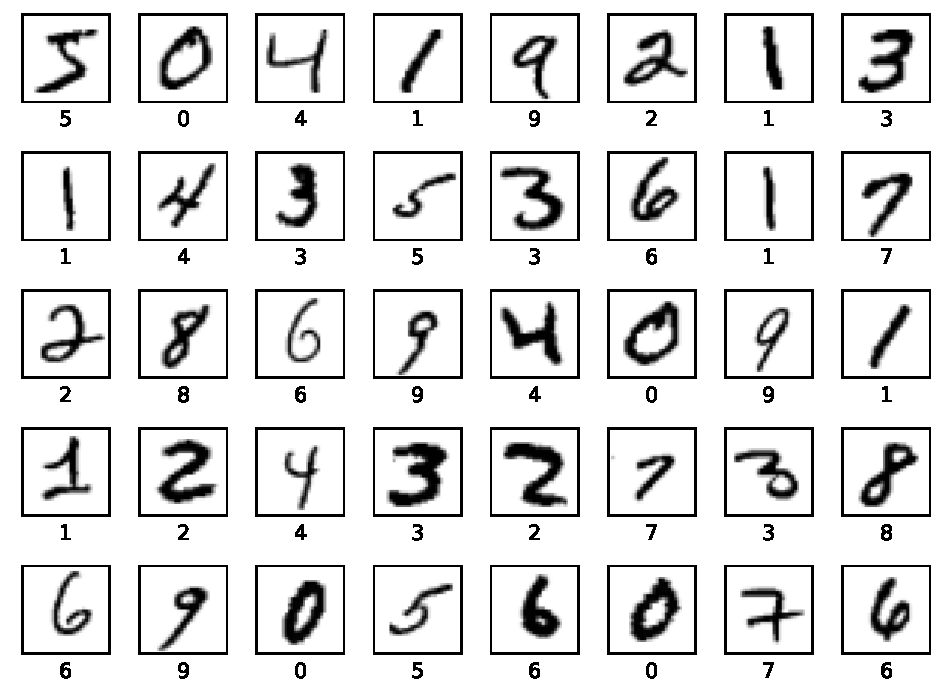
\includegraphics[width=0.6\textwidth]{chapters/Datasets/figures/MNIST.pdf}
    \fonte{From the author (2021)}
    \label{fig:dataset_mnist}
\end{figure}


\section{Fashion MNIST} \label{sec:fashion_mnist}
The simplicity of the \gls{MNIST} dataset makes it a very natural choice for benchmarking a Neural Network, however the data that it represents is also very simplistic \textbf{--} \textcite{mnistSOTA2013} were able to achieve a classification error lower than 0.3\% on the test set. The fact that \gls{MNIST} can be too easy has raised some questions about the usefulness of this dataset in benchmarking methods that scale to more complex tasks.

In response to these questions \textcite{fashionMNIST2017} proposed the Fashion MNIST dataset, arguing that \gls{MNIST} is too easy and cannot represent modern computer vision problems. Their goal was to replace \gls{MNIST} with a more robust dataset, without losing the simplicity of use that made the original so popular in the first place.

The Fashion MNIST dataset has all the same properties of \gls{MNIST}, it consists of 70,000 (60,000 training and 10,000 testing) $28{\times}28$ gray-scale images labelled from 0 to 9. The images however do not represent handwritten digits, they are instead preprocessed pictures of clothing items from the Zalando fashion company \cite{fashionMNIST2017}, the labels directly map to the type of clothing represented. Just like in \gls{MNIST}, the pixel values for the images are also inverted, the authors have made an effort to make the change of datasets as simple as just changing the link to get the files.

\autoref{fig:dataset_fashion_mnist} shows some labeled samples from this dataset, the pixel values are inverted for better visualization.
\begin{figure}[hbt]
    \centering
    \caption{Labeled samples from the Fashion MNIST dataset}
    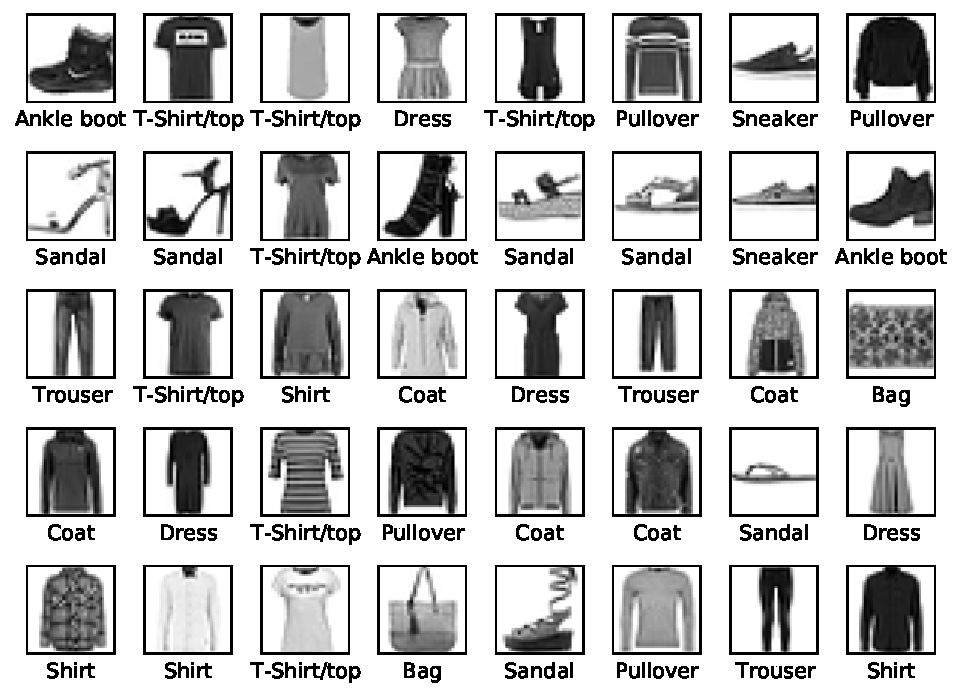
\includegraphics[width=0.7\textwidth]{chapters/Datasets/figures/Fashion_MNIST.pdf}
    \fonte{From the author (2021)}
    \label{fig:dataset_fashion_mnist}
\end{figure}


\section{CIFAR-10} \label{sec:cifar}
The \gls{CIFAR} datasets, \gls{CIFAR}-10 and \gls{CIFAR}-100, are two different subsets of the much larger 80 Million Tiny Images dataset, both are made of 60,000 (50,000 training and 10,000 testing) colored natural images of size $32{\times}32$ that were labeled by paid students to fit in a set of classes.

The images from \gls{CIFAR}-10 are divided into 10 classes with 6,000 images each, while \gls{CIFAR}-100 has 100 classes with 600 images each \cite{cifar2009}. For this document, only the \gls{CIFAR}-10 dataset was chosen for the experiments.

The \gls{CIFAR} datasets are another very popular choice for benchmarking neural networks, but given that they consist of colored images with increased resolution and more complex classes they offer considerably more challenge when compared to the \gls{MNIST} dataset. \autoref{fig:dataset_cifar10} shows examples of labeled samples taken from the \gls{CIFAR}-10 dataset.
\begin{figure}[hbt]
    \centering
    \caption{Labeled samples from CIFAR10 dataset}
    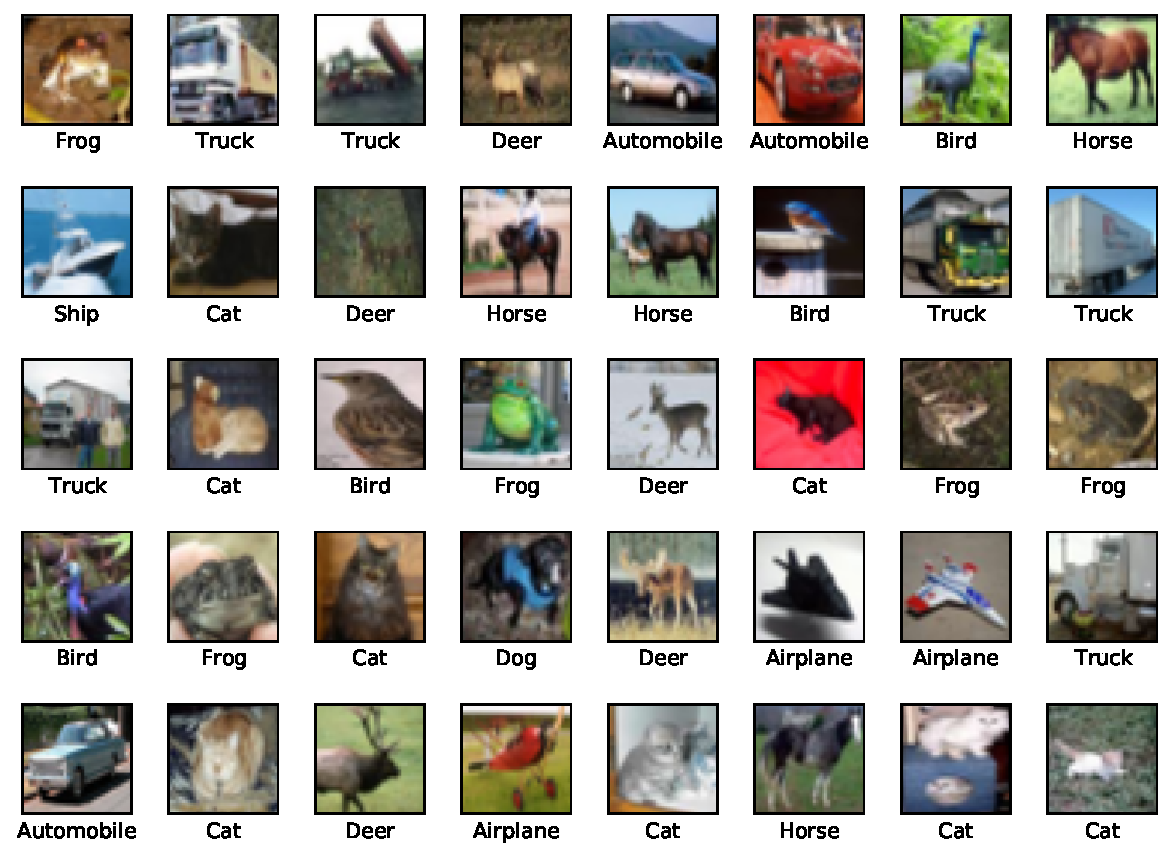
\includegraphics[width=0.7\textwidth]{chapters/Datasets/figures/CIFAR10.pdf}
    \fonte{From the author (2021)}
    \label{fig:dataset_cifar10}
\end{figure}



\section{Flowers} \label{sec:flowers}
The flowers dataset consists of $8,189$ high resolution images of 102 different categories of flowers, each category has from 40 to 250 different images \cite{flowers2008}. Samples from this dataset can be seen on \autoref{fig:dataset_flowers}

\begin{figure} [hbt]
    \centering
    \caption{Samples from the Flowers dataset}
    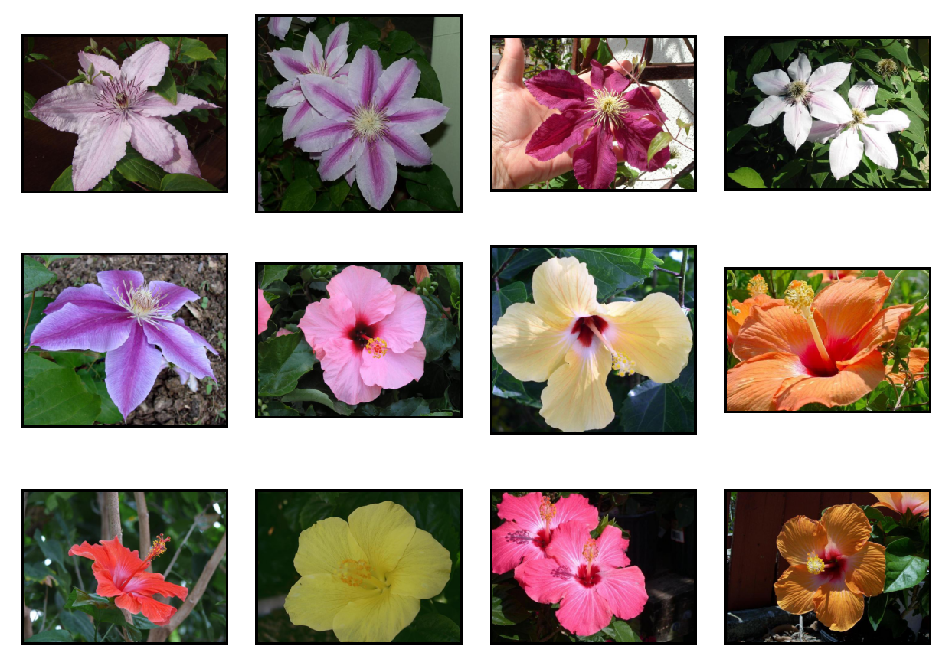
\includegraphics[width=0.8\textwidth]{chapters/Datasets/figures/Flowers.pdf}
    \fonte{From the author (2021)}
    \label{fig:dataset_flowers}
\end{figure}

\section{CelebA} \label{sec:celebA}
This is the largest dataset used in this document in terms of number of elements, it consists of $202,599$ pictures of faces of celebrities, all rescaled to size $178\times218$. All images are heavily annotated, having $40$ binary features (e.g. blonde hair, eyeglasses, wearing hat, young) and the positions of eyes, nose and mouth all labeled \cite{celebA2015}. However, for the purposes of this document the annotations will not be relevant. \autoref{fig:dataset_celeba} shows examples of pictures in this dataset.
\begin{figure}
    \centering
    \caption{Samples from the CelebA dataset}
    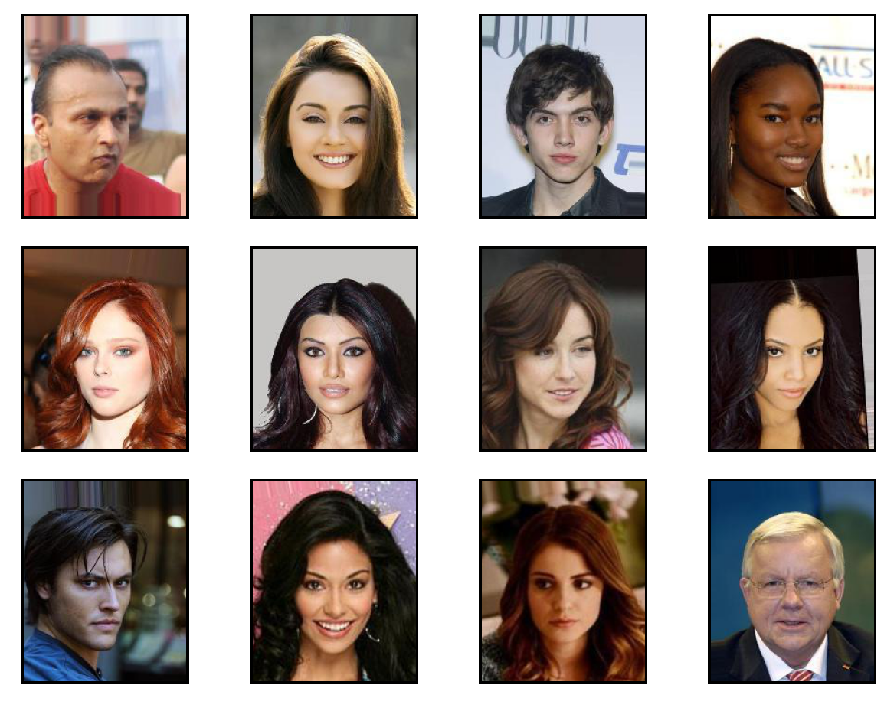
\includegraphics[width=0.8\textwidth]{chapters/Datasets/figures/CelebA.pdf}
    \fonte{From the author (2021)}
    \label{fig:dataset_celeba}
\end{figure}

\chapter{Datasets} \label{cha:datasets}
To understand the concepts explored in this document it is sometimes helpful to bring real world examples in order to represent the theoretical ideas in more familiar terms. This chapter will introduce the datasets relevant to this document, used for explaining the concepts, but mostly for performing the experiments that will be described in \autoref{cha:experiments}.

For any machine learning problem there is the desire to model something, some practical examples could be: how likely a person is to have a disease given a set of medical conditions; what type of animal an image represents; or what is the best move to make given a board position in chess. Whatever the underlying situation being modeled, it is necessary to have some data to build the model around.

This data can be obtained through self play (e.g. in Reinforcement Learning problems), but in the majority of cases it is given by a dataset. A dataset is simply a collection of samples from the situation being modeled, it does not contain all the possible values but, if sufficiently expansive, it should have enough samples to be a good representation of the distributions and particularities of the modeled situation. The goal of a dataset is to contain enough data, so that a machine learning algorithm trained on it can generalize well to data outside of it.

For neural networks a dataset is commonly divided into three groups: training, validation and test data. The training data is used in the learning process, it is what the network will see and will try to model, given this importance it is usually the largest chunk of a dataset. The validation data on the other hand is used to decide how to build the network and how to train the model, another way of saying this is that the training data is used to tune the network's parameters, while the validation data is used to tune the hyperparameters (see \autoref{sec:loss_&_gradient_descent}).

The validation process consists of training several models on the usually smaller validation data and seeing which set of hyperparameters produced the better results. One might wonder why would there be a need for this data and why not just use the training data instead? The main benefit of using a different set for validation is that validating on the training data has the risk of finding a set of hyperparameters that is particularly good on this data but that does not generalize well, using a separate validation data is a way to not overfit the hyperparameters to the training data and achieve better generalization.

The last chunk of a dataset, the test data, is used to validate the quality of the model and it's hability to generalize. This data should never be used to update either the parameters or hyperparameters, it should instead only be used as an evaluation tool, a way to estimate how well the model will perform on unseen data.

The next sections will explore the datasets relevant to the experiments made for this document. It is usual for datasets to already come separated into train and test data (the validation data is usually taken from a subset of the training data only if needed). This division will be mentioned for the described datasets, but it is relevant to note that any other divisions could also be obtained by combining and redistributing the data differently.


\section{MNIST} \label{sec:mnist}
\glsreset{MNIST}
Introduced in 1998 by \textcite{mnist1998}, the \gls{MNIST} is one of the most popular datasets in the field of machine learning, it's simplicity has made it a perfect choice as an introduction to deep learning and classification problems \cite{NN&DL2015}, but also as a benchmark for new techniques in serious research \textbf{--} some examples include \cite{dropout2012}, \cite{gans2014}, \cite{conditionalGAN2014} and \cite{adam2017}.

This dataset consists of 70,000 (60,000 training and 10,000 test) gray-scale images of handwritten digits, all images are of size $28{\times}28$ pixels and are labeled with the corresponding digit. The pixel values are inverted, this means that the strength of the strokes are represented with white pixels (values close to 255) against a black background (pixel value 0), this is however just how the data is represented numerically, for visualization purposes it is better to invert the colors as seen on \autoref{fig:dataset_mnist} \textbf{--} This figure shows some samples from this dataset along with the corresponding label.
\begin{figure}[hbt]
    \centering
    \caption{Labeled samples from the MNIST dataset}
    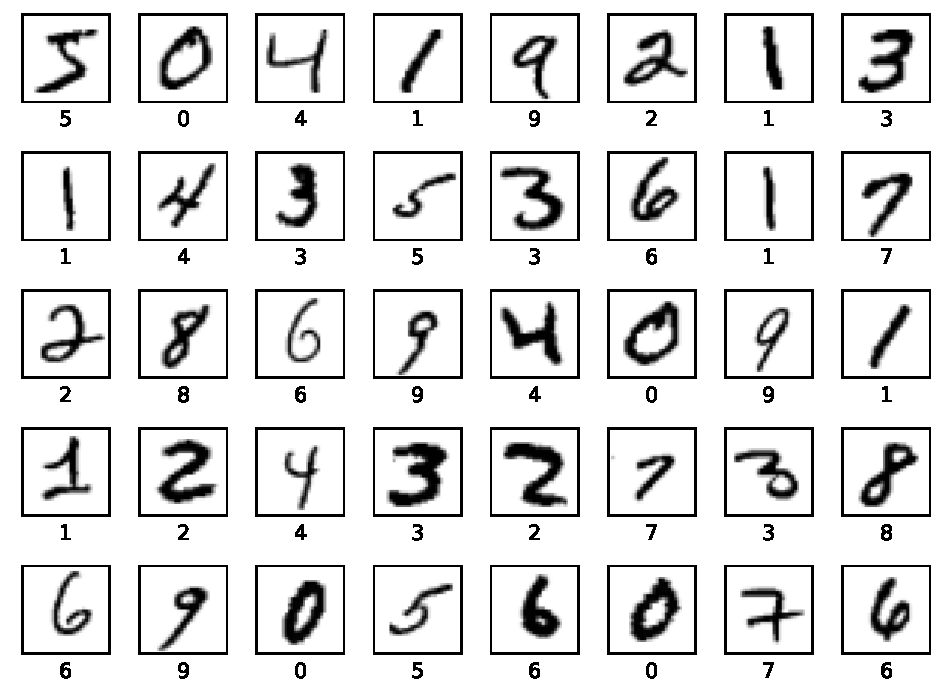
\includegraphics[width=0.6\textwidth]{chapters/Datasets/figures/MNIST.pdf}
    \fonte{From the author (2021)}
    \label{fig:dataset_mnist}
\end{figure}


\section{Fashion MNIST} \label{sec:fashion_mnist}
The simplicity of the \gls{MNIST} dataset makes it a very natural choice for benchmarking a Neural Network, however the data that it represents is also very simplistic \textbf{--} \textcite{mnistSOTA2013} were able to achieve a classification error lower than 0.3\% on the test set. The fact that \gls{MNIST} can be too easy has raised some questions about the usefulness of this dataset in benchmarking methods that scale to more complex tasks.

In response to these questions \textcite{fashionMNIST2017} proposed the Fashion MNIST dataset, arguing that \gls{MNIST} is too easy and cannot represent modern computer vision problems. Their goal was to replace \gls{MNIST} with a more robust dataset, without losing the simplicity of use that made the original so popular in the first place.

The Fashion MNIST dataset has all the same properties of \gls{MNIST}, it consists of 70,000 (60,000 training and 10,000 testing) $28{\times}28$ gray-scale images labelled from 0 to 9. The images however do not represent handwritten digits, they are instead preprocessed pictures of clothing items from the Zalando fashion company \cite{fashionMNIST2017}, the labels directly map to the type of clothing represented. Just like in \gls{MNIST}, the pixel values for the images are also inverted, the authors have made an effort to make the change of datasets as simple as just changing the link to get the files.

\autoref{fig:dataset_fashion_mnist} shows some labeled samples from this dataset, the pixel values are inverted for better visualization.
\begin{figure}[hbt]
    \centering
    \caption{Labeled samples from the Fashion MNIST dataset}
    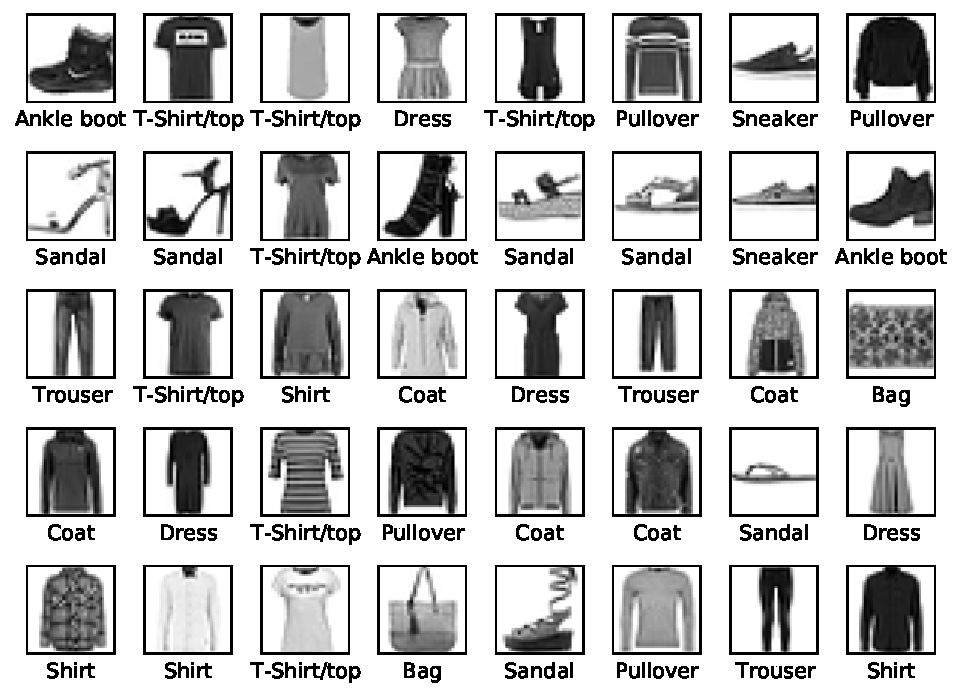
\includegraphics[width=0.7\textwidth]{chapters/Datasets/figures/Fashion_MNIST.pdf}
    \fonte{From the author (2021)}
    \label{fig:dataset_fashion_mnist}
\end{figure}


\section{CIFAR-10} \label{sec:cifar}
The \gls{CIFAR} datasets, \gls{CIFAR}-10 and \gls{CIFAR}-100, are two different subsets of the much larger 80 Million Tiny Images dataset, both are made of 60,000 (50,000 training and 10,000 testing) colored natural images of size $32{\times}32$ that were labeled by paid students to fit in a set of classes.

The images from \gls{CIFAR}-10 are divided into 10 classes with 6,000 images each, while \gls{CIFAR}-100 has 100 classes with 600 images each \cite{cifar2009}. For this document, only the \gls{CIFAR}-10 dataset was chosen for the experiments.

The \gls{CIFAR} datasets are another very popular choice for benchmarking neural networks, but given that they consist of colored images with increased resolution and more complex classes they offer considerably more challenge when compared to the \gls{MNIST} dataset. \autoref{fig:dataset_cifar10} shows examples of labeled samples taken from the \gls{CIFAR}-10 dataset.
\begin{figure}[hbt]
    \centering
    \caption{Labeled samples from CIFAR10 dataset}
    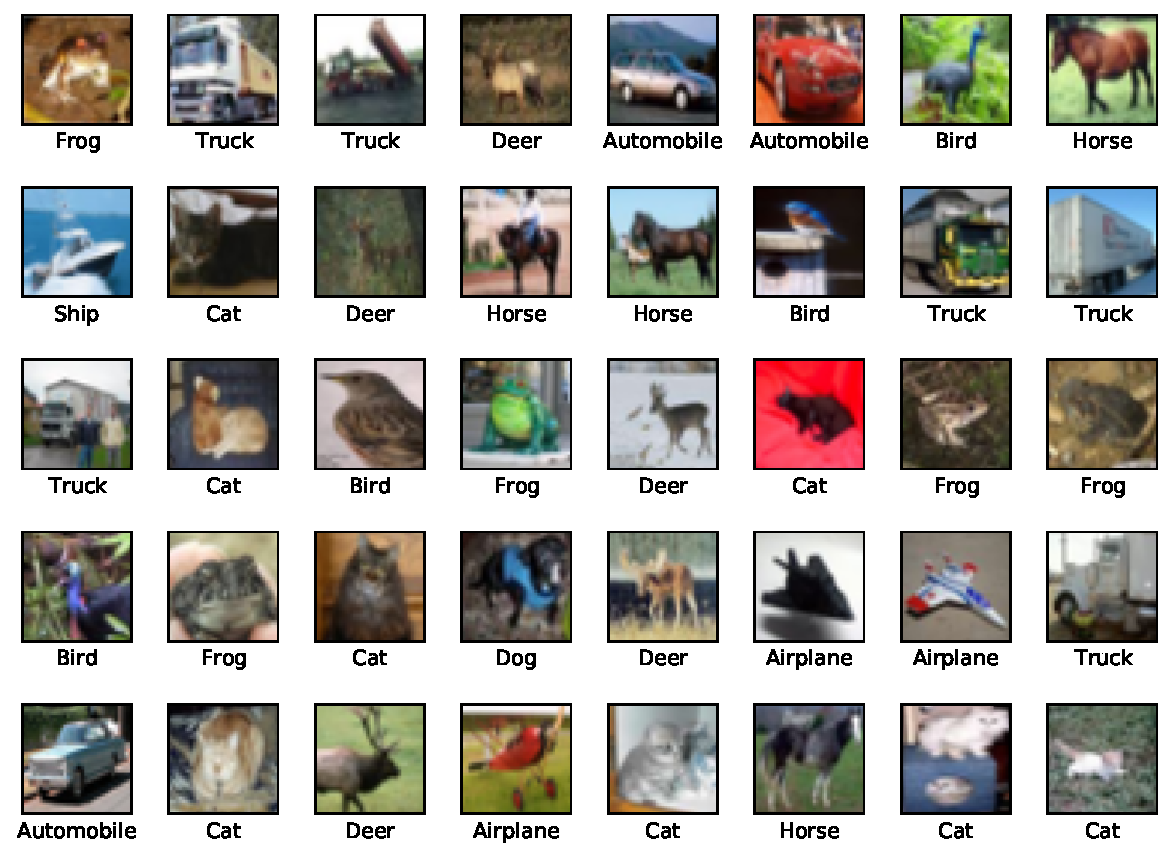
\includegraphics[width=0.7\textwidth]{chapters/Datasets/figures/CIFAR10.pdf}
    \fonte{From the author (2021)}
    \label{fig:dataset_cifar10}
\end{figure}



\section{Flowers} \label{sec:flowers}
The flowers dataset consists of $8,189$ high resolution images of 102 different categories of flowers, each category has from 40 to 250 different images \cite{flowers2008}. Samples from this dataset can be seen on \autoref{fig:dataset_flowers}

\begin{figure} [hbt]
    \centering
    \caption{Samples from the Flowers dataset}
    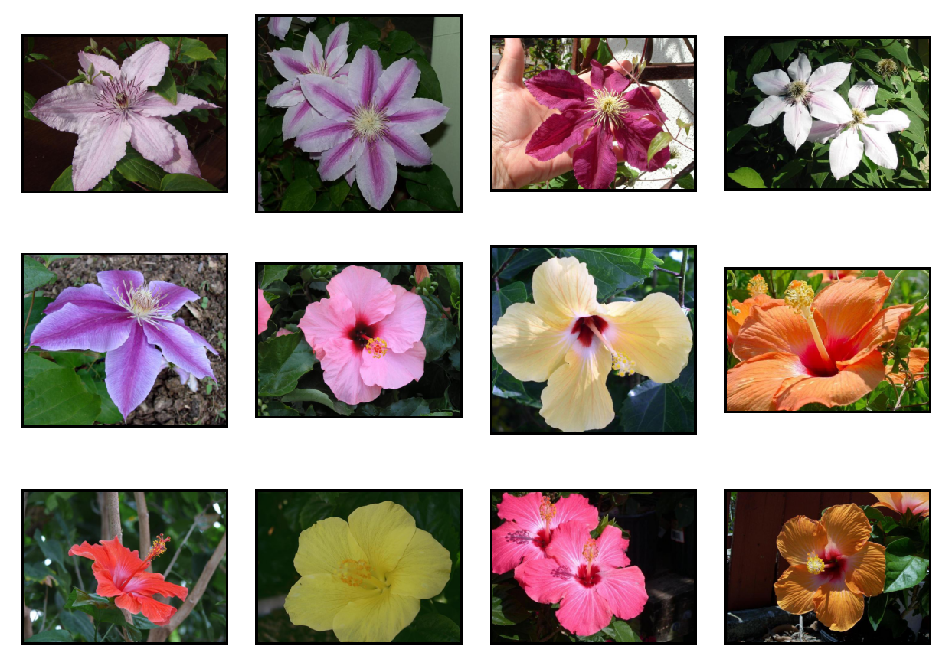
\includegraphics[width=0.8\textwidth]{chapters/Datasets/figures/Flowers.pdf}
    \fonte{From the author (2021)}
    \label{fig:dataset_flowers}
\end{figure}

\section{CelebA} \label{sec:celebA}
This is the largest dataset used in this document in terms of number of elements, it consists of $202,599$ pictures of faces of celebrities, all rescaled to size $178\times218$. All images are heavily annotated, having $40$ binary features (e.g. blonde hair, eyeglasses, wearing hat, young) and the positions of eyes, nose and mouth all labeled \cite{celebA2015}. However, for the purposes of this document the annotations will not be relevant. \autoref{fig:dataset_celeba} shows examples of pictures in this dataset.
\begin{figure}
    \centering
    \caption{Samples from the CelebA dataset}
    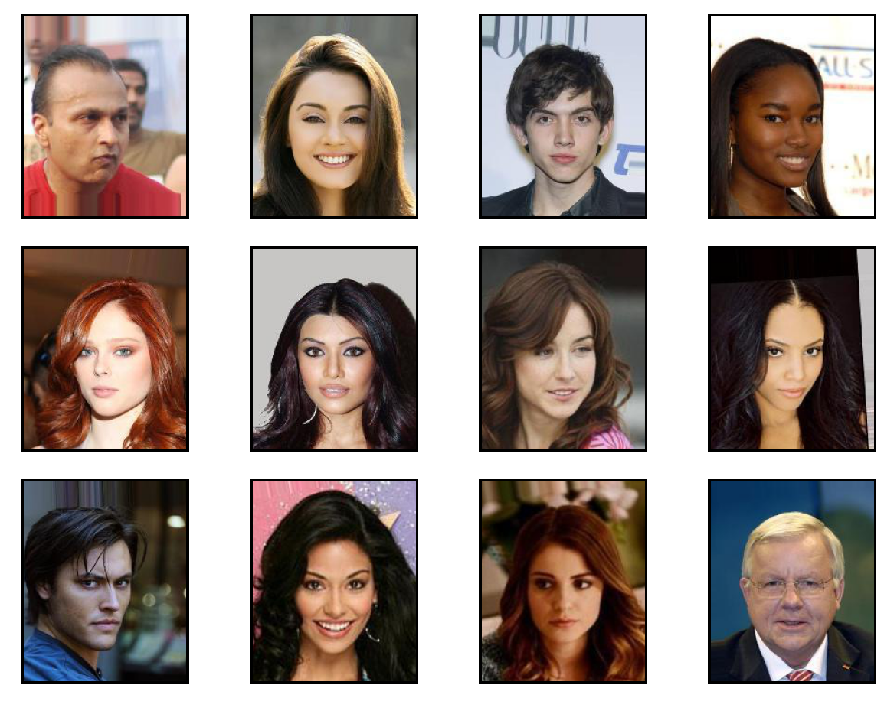
\includegraphics[width=0.8\textwidth]{chapters/Datasets/figures/CelebA.pdf}
    \fonte{From the author (2021)}
    \label{fig:dataset_celeba}
\end{figure}

\chapter{Datasets} \label{cha:datasets}
To understand the concepts explored in this document it is sometimes helpful to bring real world examples in order to represent the theoretical ideas in more familiar terms. This chapter will introduce the datasets relevant to this document, used for explaining the concepts, but mostly for performing the experiments that will be described in \autoref{cha:experiments}.

For any machine learning problem there is the desire to model something, some practical examples could be: how likely a person is to have a disease given a set of medical conditions; what type of animal an image represents; or what is the best move to make given a board position in chess. Whatever the underlying situation being modeled, it is necessary to have some data to build the model around.

This data can be obtained through self play (e.g. in Reinforcement Learning problems), but in the majority of cases it is given by a dataset. A dataset is simply a collection of samples from the situation being modeled, it does not contain all the possible values but, if sufficiently expansive, it should have enough samples to be a good representation of the distributions and particularities of the modeled situation. The goal of a dataset is to contain enough data, so that a machine learning algorithm trained on it can generalize well to data outside of it.

For neural networks a dataset is commonly divided into three groups: training, validation and test data. The training data is used in the learning process, it is what the network will see and will try to model, given this importance it is usually the largest chunk of a dataset. The validation data on the other hand is used to decide how to build the network and how to train the model, another way of saying this is that the training data is used to tune the network's parameters, while the validation data is used to tune the hyperparameters (see \autoref{sec:loss_&_gradient_descent}).

The validation process consists of training several models on the usually smaller validation data and seeing which set of hyperparameters produced the better results. One might wonder why would there be a need for this data and why not just use the training data instead? The main benefit of using a different set for validation is that validating on the training data has the risk of finding a set of hyperparameters that is particularly good on this data but that does not generalize well, using a separate validation data is a way to not overfit the hyperparameters to the training data and achieve better generalization.

The last chunk of a dataset, the test data, is used to validate the quality of the model and it's hability to generalize. This data should never be used to update either the parameters or hyperparameters, it should instead only be used as an evaluation tool, a way to estimate how well the model will perform on unseen data.

The next sections will explore the datasets relevant to the experiments made for this document. It is usual for datasets to already come separated into train and test data (the validation data is usually taken from a subset of the training data only if needed). This division will be mentioned for the described datasets, but it is relevant to note that any other divisions could also be obtained by combining and redistributing the data differently.


\section{MNIST} \label{sec:mnist}
\glsreset{MNIST}
Introduced in 1998 by \textcite{mnist1998}, the \gls{MNIST} is one of the most popular datasets in the field of machine learning, it's simplicity has made it a perfect choice as an introduction to deep learning and classification problems \cite{NN&DL2015}, but also as a benchmark for new techniques in serious research \textbf{--} some examples include \cite{dropout2012}, \cite{gans2014}, \cite{conditionalGAN2014} and \cite{adam2017}.

This dataset consists of 70,000 (60,000 training and 10,000 test) gray-scale images of handwritten digits, all images are of size $28{\times}28$ pixels and are labeled with the corresponding digit. The pixel values are inverted, this means that the strength of the strokes are represented with white pixels (values close to 255) against a black background (pixel value 0), this is however just how the data is represented numerically, for visualization purposes it is better to invert the colors as seen on \autoref{fig:dataset_mnist} \textbf{--} This figure shows some samples from this dataset along with the corresponding label.
\begin{figure}[hbt]
    \centering
    \caption{Labeled samples from the MNIST dataset}
    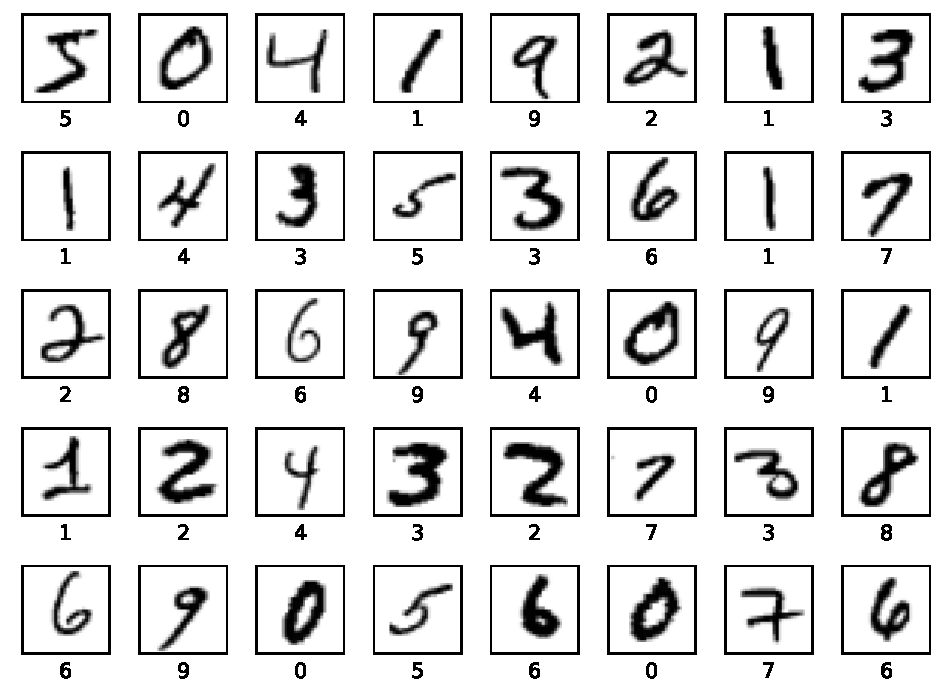
\includegraphics[width=0.6\textwidth]{chapters/Datasets/figures/MNIST.pdf}
    \fonte{From the author (2021)}
    \label{fig:dataset_mnist}
\end{figure}


\section{Fashion MNIST} \label{sec:fashion_mnist}
The simplicity of the \gls{MNIST} dataset makes it a very natural choice for benchmarking a Neural Network, however the data that it represents is also very simplistic \textbf{--} \textcite{mnistSOTA2013} were able to achieve a classification error lower than 0.3\% on the test set. The fact that \gls{MNIST} can be too easy has raised some questions about the usefulness of this dataset in benchmarking methods that scale to more complex tasks.

In response to these questions \textcite{fashionMNIST2017} proposed the Fashion MNIST dataset, arguing that \gls{MNIST} is too easy and cannot represent modern computer vision problems. Their goal was to replace \gls{MNIST} with a more robust dataset, without losing the simplicity of use that made the original so popular in the first place.

The Fashion MNIST dataset has all the same properties of \gls{MNIST}, it consists of 70,000 (60,000 training and 10,000 testing) $28{\times}28$ gray-scale images labelled from 0 to 9. The images however do not represent handwritten digits, they are instead preprocessed pictures of clothing items from the Zalando fashion company \cite{fashionMNIST2017}, the labels directly map to the type of clothing represented. Just like in \gls{MNIST}, the pixel values for the images are also inverted, the authors have made an effort to make the change of datasets as simple as just changing the link to get the files.

\autoref{fig:dataset_fashion_mnist} shows some labeled samples from this dataset, the pixel values are inverted for better visualization.
\begin{figure}[hbt]
    \centering
    \caption{Labeled samples from the Fashion MNIST dataset}
    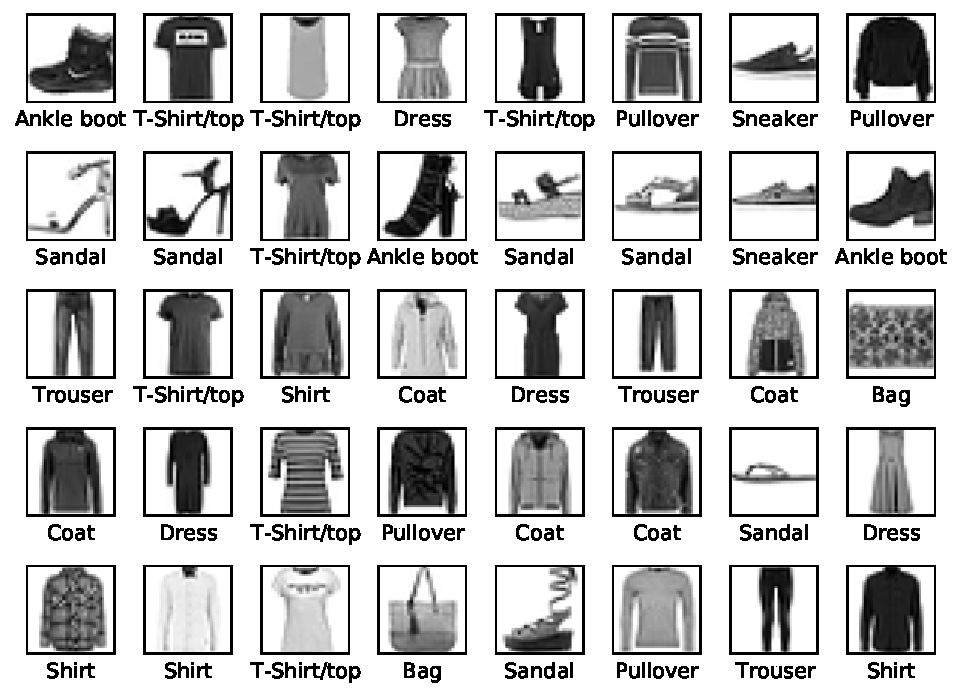
\includegraphics[width=0.7\textwidth]{chapters/Datasets/figures/Fashion_MNIST.pdf}
    \fonte{From the author (2021)}
    \label{fig:dataset_fashion_mnist}
\end{figure}


\section{CIFAR-10} \label{sec:cifar}
The \gls{CIFAR} datasets, \gls{CIFAR}-10 and \gls{CIFAR}-100, are two different subsets of the much larger 80 Million Tiny Images dataset, both are made of 60,000 (50,000 training and 10,000 testing) colored natural images of size $32{\times}32$ that were labeled by paid students to fit in a set of classes.

The images from \gls{CIFAR}-10 are divided into 10 classes with 6,000 images each, while \gls{CIFAR}-100 has 100 classes with 600 images each \cite{cifar2009}. For this document, only the \gls{CIFAR}-10 dataset was chosen for the experiments.

The \gls{CIFAR} datasets are another very popular choice for benchmarking neural networks, but given that they consist of colored images with increased resolution and more complex classes they offer considerably more challenge when compared to the \gls{MNIST} dataset. \autoref{fig:dataset_cifar10} shows examples of labeled samples taken from the \gls{CIFAR}-10 dataset.
\begin{figure}[hbt]
    \centering
    \caption{Labeled samples from CIFAR10 dataset}
    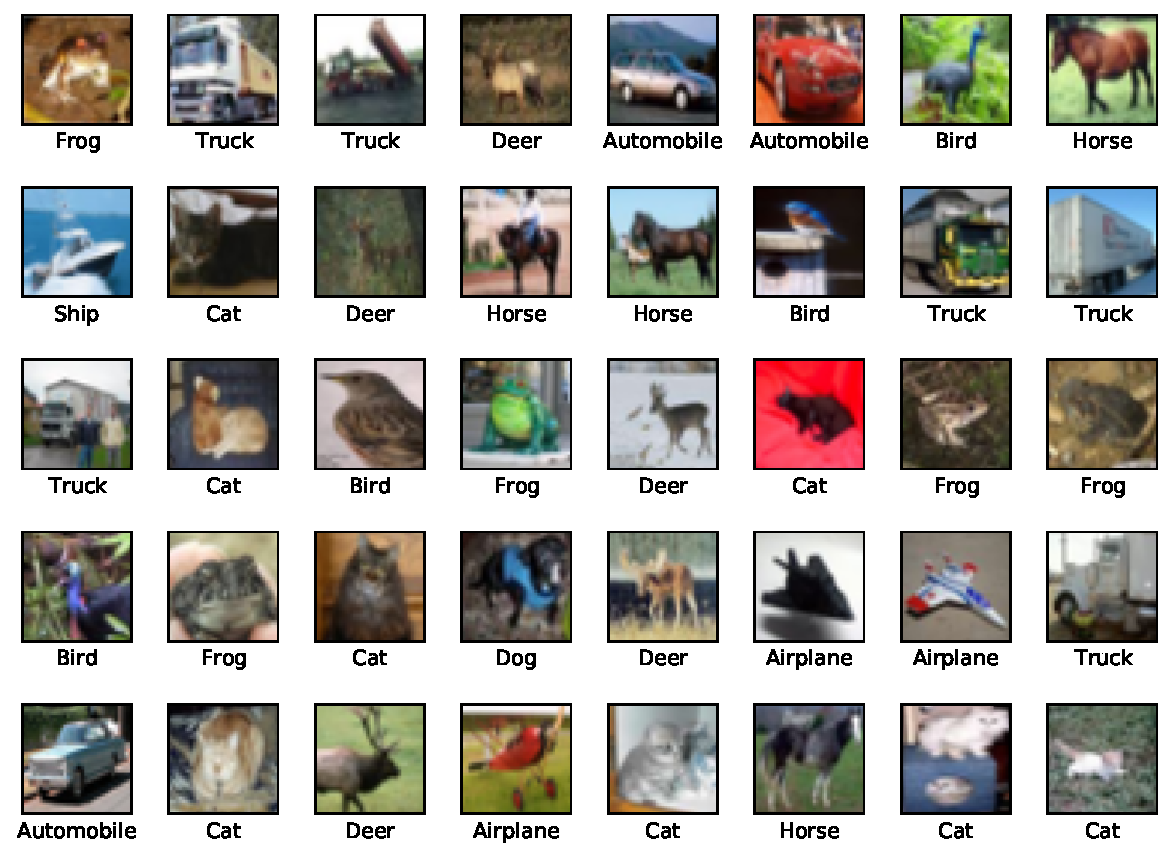
\includegraphics[width=0.7\textwidth]{chapters/Datasets/figures/CIFAR10.pdf}
    \fonte{From the author (2021)}
    \label{fig:dataset_cifar10}
\end{figure}



\section{Flowers} \label{sec:flowers}
The flowers dataset consists of $8,189$ high resolution images of 102 different categories of flowers, each category has from 40 to 250 different images \cite{flowers2008}. Samples from this dataset can be seen on \autoref{fig:dataset_flowers}

\begin{figure} [hbt]
    \centering
    \caption{Samples from the Flowers dataset}
    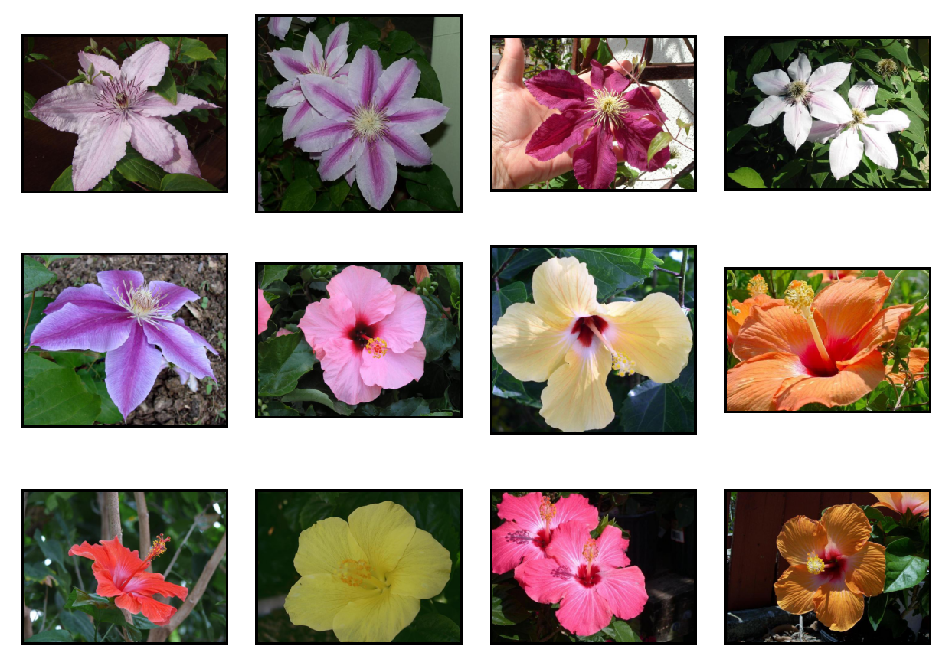
\includegraphics[width=0.8\textwidth]{chapters/Datasets/figures/Flowers.pdf}
    \fonte{From the author (2021)}
    \label{fig:dataset_flowers}
\end{figure}

\section{CelebA} \label{sec:celebA}
This is the largest dataset used in this document in terms of number of elements, it consists of $202,599$ pictures of faces of celebrities, all rescaled to size $178\times218$. All images are heavily annotated, having $40$ binary features (e.g. blonde hair, eyeglasses, wearing hat, young) and the positions of eyes, nose and mouth all labeled \cite{celebA2015}. However, for the purposes of this document the annotations will not be relevant. \autoref{fig:dataset_celeba} shows examples of pictures in this dataset.
\begin{figure}
    \centering
    \caption{Samples from the CelebA dataset}
    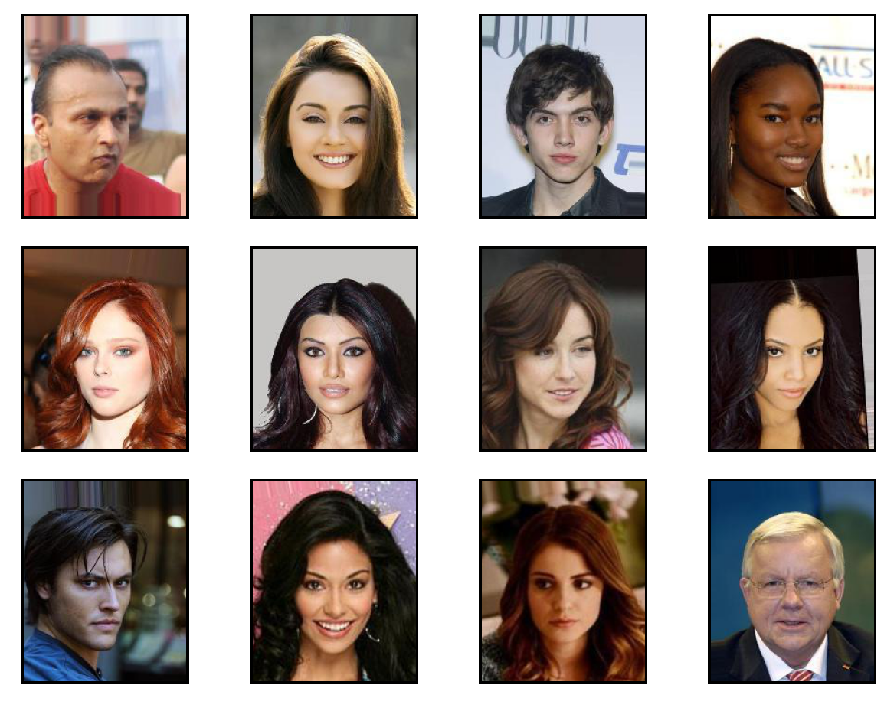
\includegraphics[width=0.8\textwidth]{chapters/Datasets/figures/CelebA.pdf}
    \fonte{From the author (2021)}
    \label{fig:dataset_celeba}
\end{figure}

\chapter{Datasets} \label{cha:datasets}
To understand the concepts explored in this document it is sometimes helpful to bring real world examples in order to represent the theoretical ideas in more familiar terms. This chapter will introduce the datasets relevant to this document, used for explaining the concepts, but mostly for performing the experiments that will be described in \autoref{cha:experiments}.

For any machine learning problem there is the desire to model something, some practical examples could be: how likely a person is to have a disease given a set of medical conditions; what type of animal an image represents; or what is the best move to make given a board position in chess. Whatever the underlying situation being modeled, it is necessary to have some data to build the model around.

This data can be obtained through self play (e.g. in Reinforcement Learning problems), but in the majority of cases it is given by a dataset. A dataset is simply a collection of samples from the situation being modeled, it does not contain all the possible values but, if sufficiently expansive, it should have enough samples to be a good representation of the distributions and particularities of the modeled situation. The goal of a dataset is to contain enough data, so that a machine learning algorithm trained on it can generalize well to data outside of it.

For neural networks a dataset is commonly divided into three groups: training, validation and test data. The training data is used in the learning process, it is what the network will see and will try to model, given this importance it is usually the largest chunk of a dataset. The validation data on the other hand is used to decide how to build the network and how to train the model, another way of saying this is that the training data is used to tune the network's parameters, while the validation data is used to tune the hyperparameters (see \autoref{sec:loss_&_gradient_descent}).

The validation process consists of training several models on the usually smaller validation data and seeing which set of hyperparameters produced the better results. One might wonder why would there be a need for this data and why not just use the training data instead? The main benefit of using a different set for validation is that validating on the training data has the risk of finding a set of hyperparameters that is particularly good on this data but that does not generalize well, using a separate validation data is a way to not overfit the hyperparameters to the training data and achieve better generalization.

The last chunk of a dataset, the test data, is used to validate the quality of the model and it's hability to generalize. This data should never be used to update either the parameters or hyperparameters, it should instead only be used as an evaluation tool, a way to estimate how well the model will perform on unseen data.

The next sections will explore the datasets relevant to the experiments made for this document. It is usual for datasets to already come separated into train and test data (the validation data is usually taken from a subset of the training data only if needed). This division will be mentioned for the described datasets, but it is relevant to note that any other divisions could also be obtained by combining and redistributing the data differently.


\section{MNIST} \label{sec:mnist}
\glsreset{MNIST}
Introduced in 1998 by \textcite{mnist1998}, the \gls{MNIST} is one of the most popular datasets in the field of machine learning, it's simplicity has made it a perfect choice as an introduction to deep learning and classification problems \cite{NN&DL2015}, but also as a benchmark for new techniques in serious research \textbf{--} some examples include \cite{dropout2012}, \cite{gans2014}, \cite{conditionalGAN2014} and \cite{adam2017}.

This dataset consists of 70,000 (60,000 training and 10,000 test) gray-scale images of handwritten digits, all images are of size $28{\times}28$ pixels and are labeled with the corresponding digit. The pixel values are inverted, this means that the strength of the strokes are represented with white pixels (values close to 255) against a black background (pixel value 0), this is however just how the data is represented numerically, for visualization purposes it is better to invert the colors as seen on \autoref{fig:dataset_mnist} \textbf{--} This figure shows some samples from this dataset along with the corresponding label.
\begin{figure}[hbt]
    \centering
    \caption{Labeled samples from the MNIST dataset}
    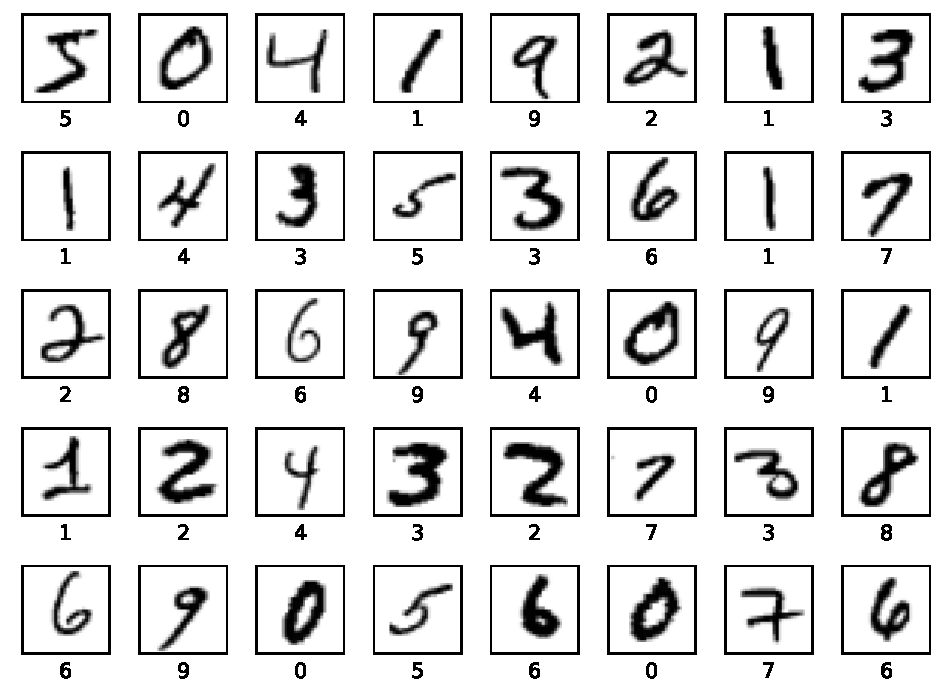
\includegraphics[width=0.6\textwidth]{chapters/Datasets/figures/MNIST.pdf}
    \fonte{From the author (2021)}
    \label{fig:dataset_mnist}
\end{figure}


\section{Fashion MNIST} \label{sec:fashion_mnist}
The simplicity of the \gls{MNIST} dataset makes it a very natural choice for benchmarking a Neural Network, however the data that it represents is also very simplistic \textbf{--} \textcite{mnistSOTA2013} were able to achieve a classification error lower than 0.3\% on the test set. The fact that \gls{MNIST} can be too easy has raised some questions about the usefulness of this dataset in benchmarking methods that scale to more complex tasks.

In response to these questions \textcite{fashionMNIST2017} proposed the Fashion MNIST dataset, arguing that \gls{MNIST} is too easy and cannot represent modern computer vision problems. Their goal was to replace \gls{MNIST} with a more robust dataset, without losing the simplicity of use that made the original so popular in the first place.

The Fashion MNIST dataset has all the same properties of \gls{MNIST}, it consists of 70,000 (60,000 training and 10,000 testing) $28{\times}28$ gray-scale images labelled from 0 to 9. The images however do not represent handwritten digits, they are instead preprocessed pictures of clothing items from the Zalando fashion company \cite{fashionMNIST2017}, the labels directly map to the type of clothing represented. Just like in \gls{MNIST}, the pixel values for the images are also inverted, the authors have made an effort to make the change of datasets as simple as just changing the link to get the files.

\autoref{fig:dataset_fashion_mnist} shows some labeled samples from this dataset, the pixel values are inverted for better visualization.
\begin{figure}[hbt]
    \centering
    \caption{Labeled samples from the Fashion MNIST dataset}
    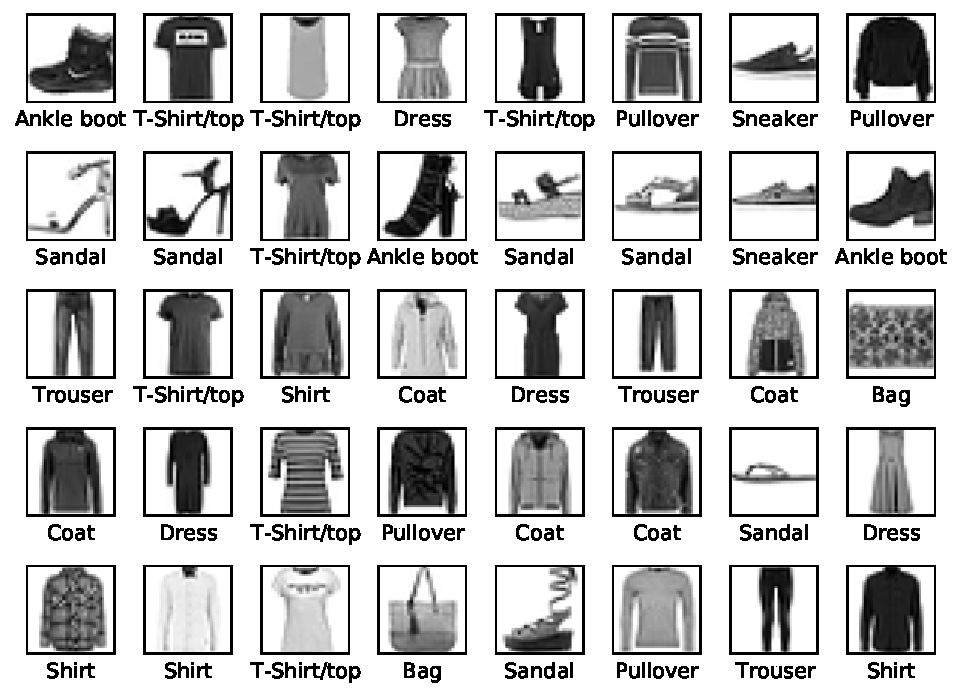
\includegraphics[width=0.7\textwidth]{chapters/Datasets/figures/Fashion_MNIST.pdf}
    \fonte{From the author (2021)}
    \label{fig:dataset_fashion_mnist}
\end{figure}


\section{CIFAR-10} \label{sec:cifar}
The \gls{CIFAR} datasets, \gls{CIFAR}-10 and \gls{CIFAR}-100, are two different subsets of the much larger 80 Million Tiny Images dataset, both are made of 60,000 (50,000 training and 10,000 testing) colored natural images of size $32{\times}32$ that were labeled by paid students to fit in a set of classes.

The images from \gls{CIFAR}-10 are divided into 10 classes with 6,000 images each, while \gls{CIFAR}-100 has 100 classes with 600 images each \cite{cifar2009}. For this document, only the \gls{CIFAR}-10 dataset was chosen for the experiments.

The \gls{CIFAR} datasets are another very popular choice for benchmarking neural networks, but given that they consist of colored images with increased resolution and more complex classes they offer considerably more challenge when compared to the \gls{MNIST} dataset. \autoref{fig:dataset_cifar10} shows examples of labeled samples taken from the \gls{CIFAR}-10 dataset.
\begin{figure}[hbt]
    \centering
    \caption{Labeled samples from CIFAR10 dataset}
    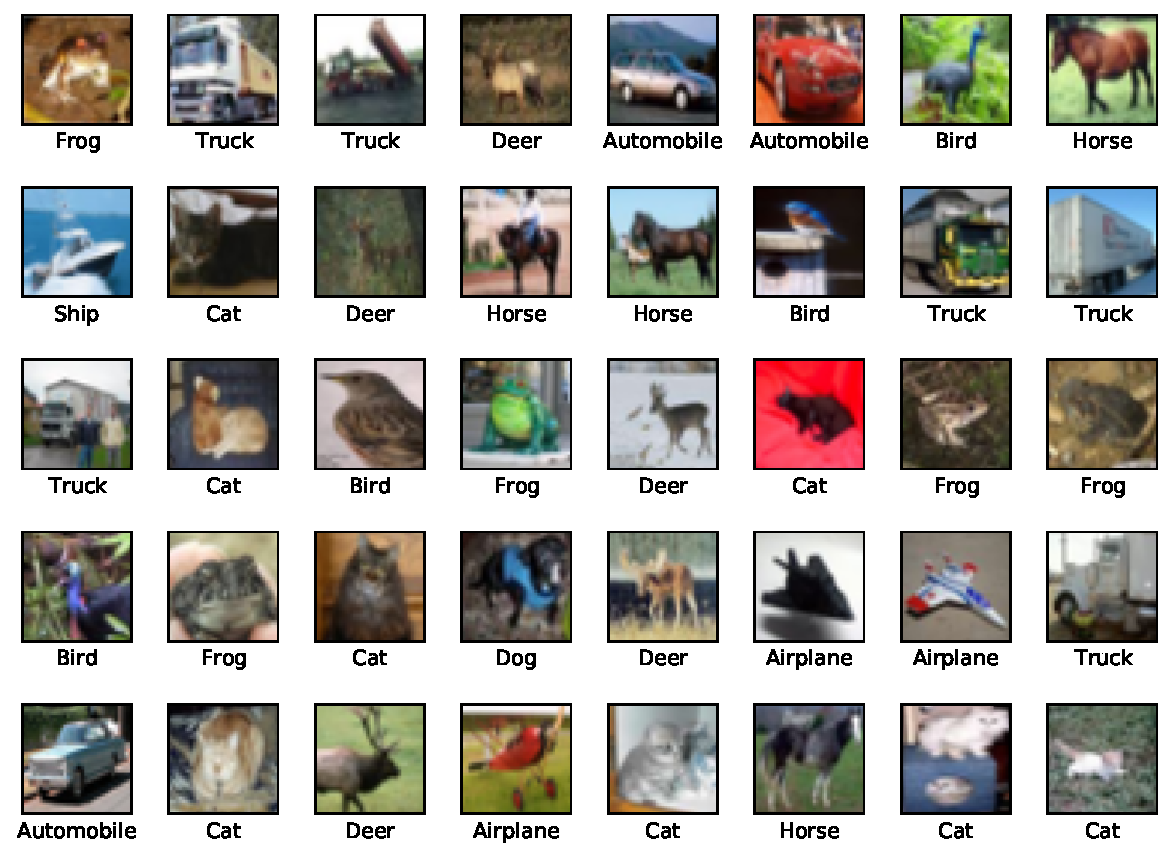
\includegraphics[width=0.7\textwidth]{chapters/Datasets/figures/CIFAR10.pdf}
    \fonte{From the author (2021)}
    \label{fig:dataset_cifar10}
\end{figure}



\section{Flowers} \label{sec:flowers}
The flowers dataset consists of $8,189$ high resolution images of 102 different categories of flowers, each category has from 40 to 250 different images \cite{flowers2008}. Samples from this dataset can be seen on \autoref{fig:dataset_flowers}

\begin{figure} [hbt]
    \centering
    \caption{Samples from the Flowers dataset}
    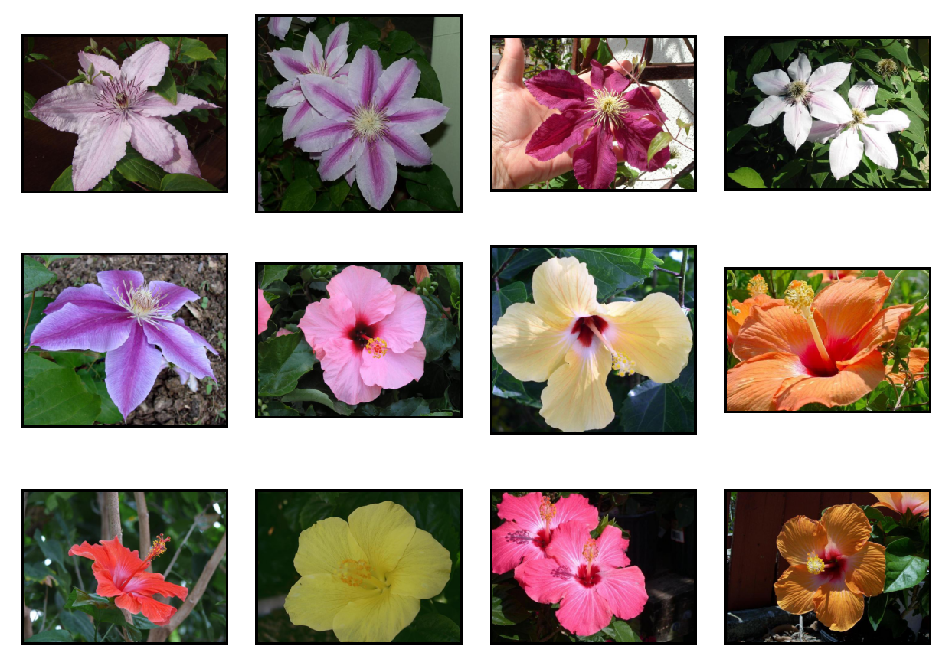
\includegraphics[width=0.8\textwidth]{chapters/Datasets/figures/Flowers.pdf}
    \fonte{From the author (2021)}
    \label{fig:dataset_flowers}
\end{figure}

\section{CelebA} \label{sec:celebA}
This is the largest dataset used in this document in terms of number of elements, it consists of $202,599$ pictures of faces of celebrities, all rescaled to size $178\times218$. All images are heavily annotated, having $40$ binary features (e.g. blonde hair, eyeglasses, wearing hat, young) and the positions of eyes, nose and mouth all labeled \cite{celebA2015}. However, for the purposes of this document the annotations will not be relevant. \autoref{fig:dataset_celeba} shows examples of pictures in this dataset.
\begin{figure}
    \centering
    \caption{Samples from the CelebA dataset}
    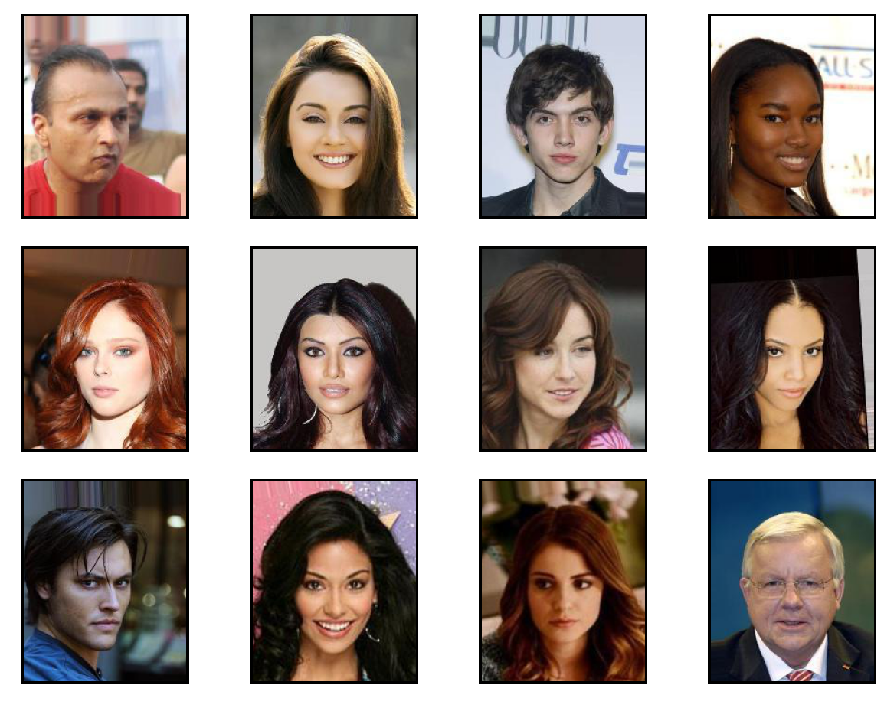
\includegraphics[width=0.8\textwidth]{chapters/Datasets/figures/CelebA.pdf}
    \fonte{From the author (2021)}
    \label{fig:dataset_celeba}
\end{figure}

\chapter{Datasets} \label{cha:datasets}
To understand the concepts explored in this document it is sometimes helpful to bring real world examples in order to represent the theoretical ideas in more familiar terms. This chapter will introduce the datasets relevant to this document, used for explaining the concepts, but mostly for performing the experiments that will be described in \autoref{cha:experiments}.

For any machine learning problem there is the desire to model something, some practical examples could be: how likely a person is to have a disease given a set of medical conditions; what type of animal an image represents; or what is the best move to make given a board position in chess. Whatever the underlying situation being modeled, it is necessary to have some data to build the model around.

This data can be obtained through self play (e.g. in Reinforcement Learning problems), but in the majority of cases it is given by a dataset. A dataset is simply a collection of samples from the situation being modeled, it does not contain all the possible values but, if sufficiently expansive, it should have enough samples to be a good representation of the distributions and particularities of the modeled situation. The goal of a dataset is to contain enough data, so that a machine learning algorithm trained on it can generalize well to data outside of it.

For neural networks a dataset is commonly divided into three groups: training, validation and test data. The training data is used in the learning process, it is what the network will see and will try to model, given this importance it is usually the largest chunk of a dataset. The validation data on the other hand is used to decide how to build the network and how to train the model, another way of saying this is that the training data is used to tune the network's parameters, while the validation data is used to tune the hyperparameters (see \autoref{sec:loss_&_gradient_descent}).

The validation process consists of training several models on the usually smaller validation data and seeing which set of hyperparameters produced the better results. One might wonder why would there be a need for this data and why not just use the training data instead? The main benefit of using a different set for validation is that validating on the training data has the risk of finding a set of hyperparameters that is particularly good on this data but that does not generalize well, using a separate validation data is a way to not overfit the hyperparameters to the training data and achieve better generalization.

The last chunk of a dataset, the test data, is used to validate the quality of the model and it's hability to generalize. This data should never be used to update either the parameters or hyperparameters, it should instead only be used as an evaluation tool, a way to estimate how well the model will perform on unseen data.

The next sections will explore the datasets relevant to the experiments made for this document. It is usual for datasets to already come separated into train and test data (the validation data is usually taken from a subset of the training data only if needed). This division will be mentioned for the described datasets, but it is relevant to note that any other divisions could also be obtained by combining and redistributing the data differently.


\section{MNIST} \label{sec:mnist}
\glsreset{MNIST}
Introduced in 1998 by \textcite{mnist1998}, the \gls{MNIST} is one of the most popular datasets in the field of machine learning, it's simplicity has made it a perfect choice as an introduction to deep learning and classification problems \cite{NN&DL2015}, but also as a benchmark for new techniques in serious research \textbf{--} some examples include \cite{dropout2012}, \cite{gans2014}, \cite{conditionalGAN2014} and \cite{adam2017}.

This dataset consists of 70,000 (60,000 training and 10,000 test) gray-scale images of handwritten digits, all images are of size $28{\times}28$ pixels and are labeled with the corresponding digit. The pixel values are inverted, this means that the strength of the strokes are represented with white pixels (values close to 255) against a black background (pixel value 0), this is however just how the data is represented numerically, for visualization purposes it is better to invert the colors as seen on \autoref{fig:dataset_mnist} \textbf{--} This figure shows some samples from this dataset along with the corresponding label.
\begin{figure}[hbt]
    \centering
    \caption{Labeled samples from the MNIST dataset}
    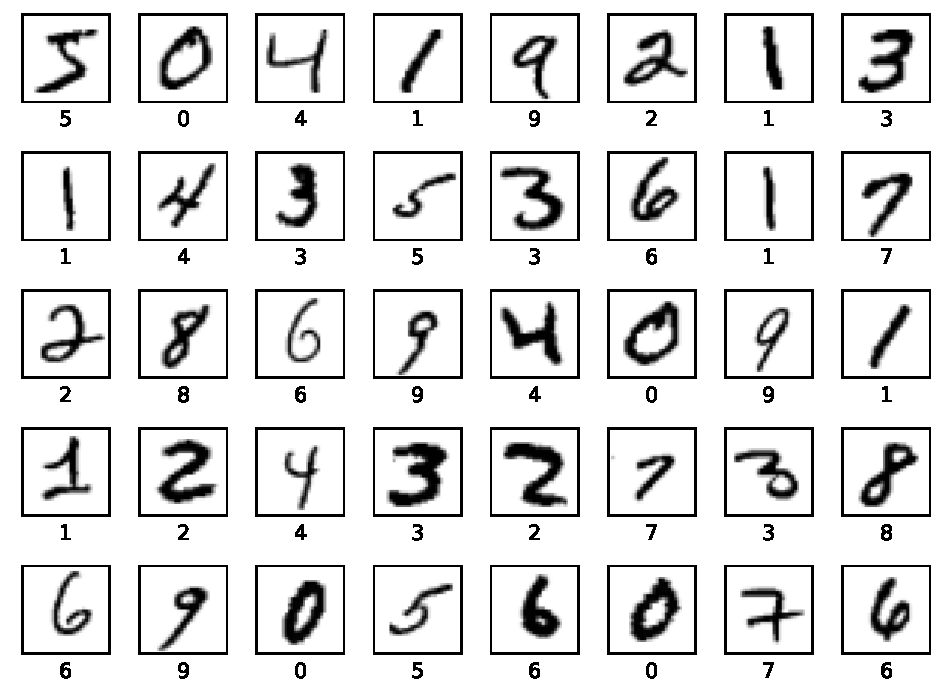
\includegraphics[width=0.6\textwidth]{chapters/Datasets/figures/MNIST.pdf}
    \fonte{From the author (2021)}
    \label{fig:dataset_mnist}
\end{figure}


\section{Fashion MNIST} \label{sec:fashion_mnist}
The simplicity of the \gls{MNIST} dataset makes it a very natural choice for benchmarking a Neural Network, however the data that it represents is also very simplistic \textbf{--} \textcite{mnistSOTA2013} were able to achieve a classification error lower than 0.3\% on the test set. The fact that \gls{MNIST} can be too easy has raised some questions about the usefulness of this dataset in benchmarking methods that scale to more complex tasks.

In response to these questions \textcite{fashionMNIST2017} proposed the Fashion MNIST dataset, arguing that \gls{MNIST} is too easy and cannot represent modern computer vision problems. Their goal was to replace \gls{MNIST} with a more robust dataset, without losing the simplicity of use that made the original so popular in the first place.

The Fashion MNIST dataset has all the same properties of \gls{MNIST}, it consists of 70,000 (60,000 training and 10,000 testing) $28{\times}28$ gray-scale images labelled from 0 to 9. The images however do not represent handwritten digits, they are instead preprocessed pictures of clothing items from the Zalando fashion company \cite{fashionMNIST2017}, the labels directly map to the type of clothing represented. Just like in \gls{MNIST}, the pixel values for the images are also inverted, the authors have made an effort to make the change of datasets as simple as just changing the link to get the files.

\autoref{fig:dataset_fashion_mnist} shows some labeled samples from this dataset, the pixel values are inverted for better visualization.
\begin{figure}[hbt]
    \centering
    \caption{Labeled samples from the Fashion MNIST dataset}
    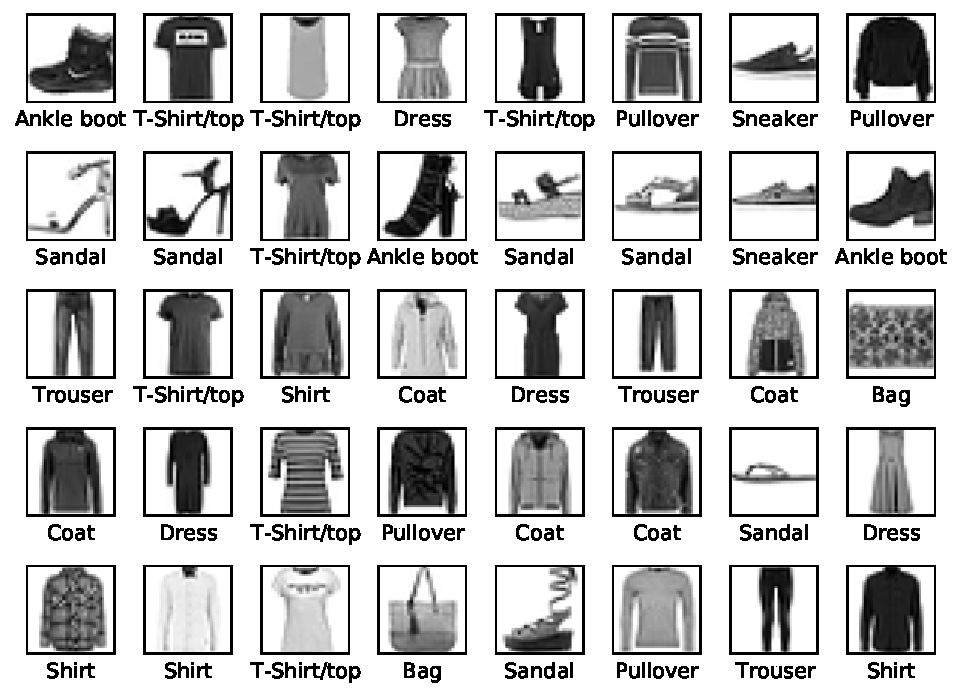
\includegraphics[width=0.7\textwidth]{chapters/Datasets/figures/Fashion_MNIST.pdf}
    \fonte{From the author (2021)}
    \label{fig:dataset_fashion_mnist}
\end{figure}


\section{CIFAR-10} \label{sec:cifar}
The \gls{CIFAR} datasets, \gls{CIFAR}-10 and \gls{CIFAR}-100, are two different subsets of the much larger 80 Million Tiny Images dataset, both are made of 60,000 (50,000 training and 10,000 testing) colored natural images of size $32{\times}32$ that were labeled by paid students to fit in a set of classes.

The images from \gls{CIFAR}-10 are divided into 10 classes with 6,000 images each, while \gls{CIFAR}-100 has 100 classes with 600 images each \cite{cifar2009}. For this document, only the \gls{CIFAR}-10 dataset was chosen for the experiments.

The \gls{CIFAR} datasets are another very popular choice for benchmarking neural networks, but given that they consist of colored images with increased resolution and more complex classes they offer considerably more challenge when compared to the \gls{MNIST} dataset. \autoref{fig:dataset_cifar10} shows examples of labeled samples taken from the \gls{CIFAR}-10 dataset.
\begin{figure}[hbt]
    \centering
    \caption{Labeled samples from CIFAR10 dataset}
    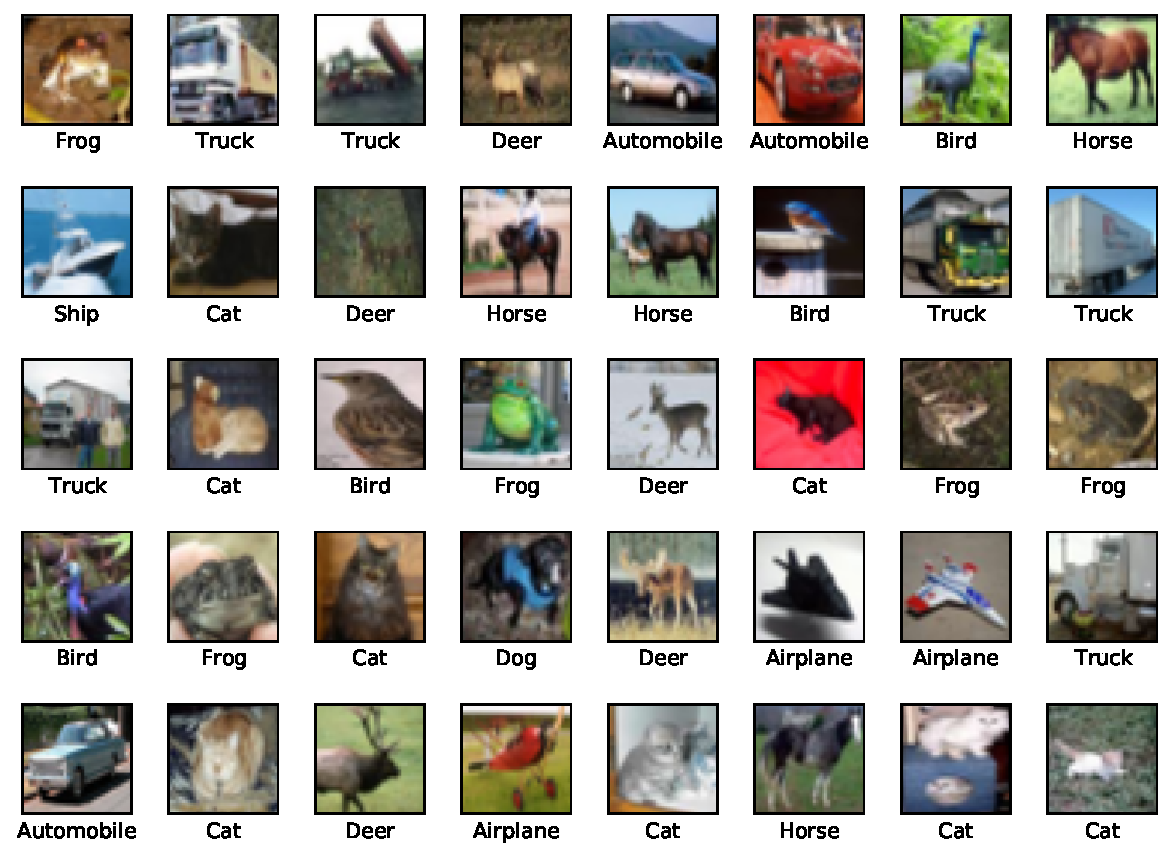
\includegraphics[width=0.7\textwidth]{chapters/Datasets/figures/CIFAR10.pdf}
    \fonte{From the author (2021)}
    \label{fig:dataset_cifar10}
\end{figure}



\section{Flowers} \label{sec:flowers}
The flowers dataset consists of $8,189$ high resolution images of 102 different categories of flowers, each category has from 40 to 250 different images \cite{flowers2008}. Samples from this dataset can be seen on \autoref{fig:dataset_flowers}

\begin{figure} [hbt]
    \centering
    \caption{Samples from the Flowers dataset}
    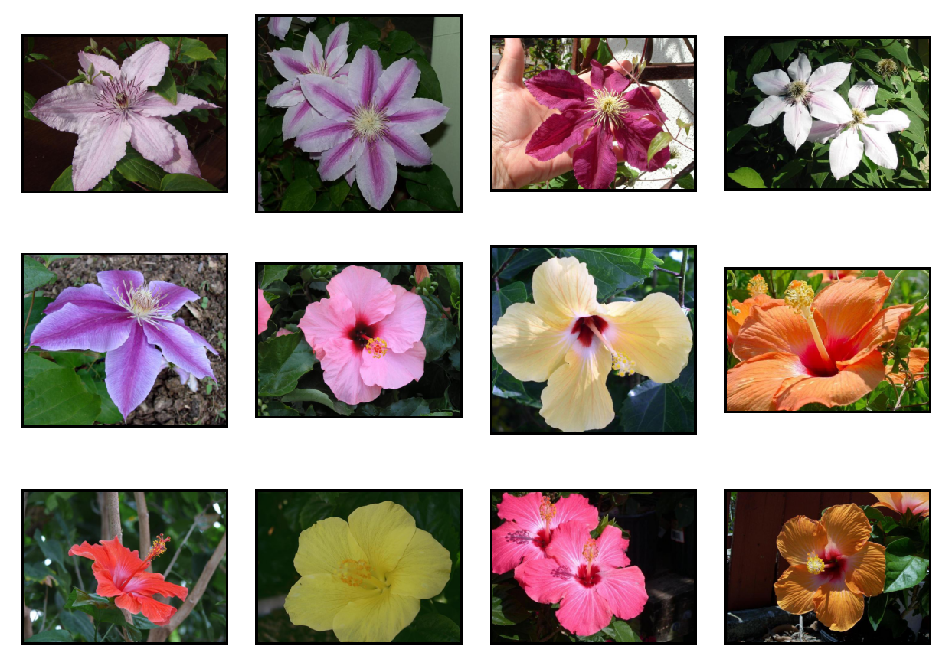
\includegraphics[width=0.8\textwidth]{chapters/Datasets/figures/Flowers.pdf}
    \fonte{From the author (2021)}
    \label{fig:dataset_flowers}
\end{figure}

\section{CelebA} \label{sec:celebA}
This is the largest dataset used in this document in terms of number of elements, it consists of $202,599$ pictures of faces of celebrities, all rescaled to size $178\times218$. All images are heavily annotated, having $40$ binary features (e.g. blonde hair, eyeglasses, wearing hat, young) and the positions of eyes, nose and mouth all labeled \cite{celebA2015}. However, for the purposes of this document the annotations will not be relevant. \autoref{fig:dataset_celeba} shows examples of pictures in this dataset.
\begin{figure}
    \centering
    \caption{Samples from the CelebA dataset}
    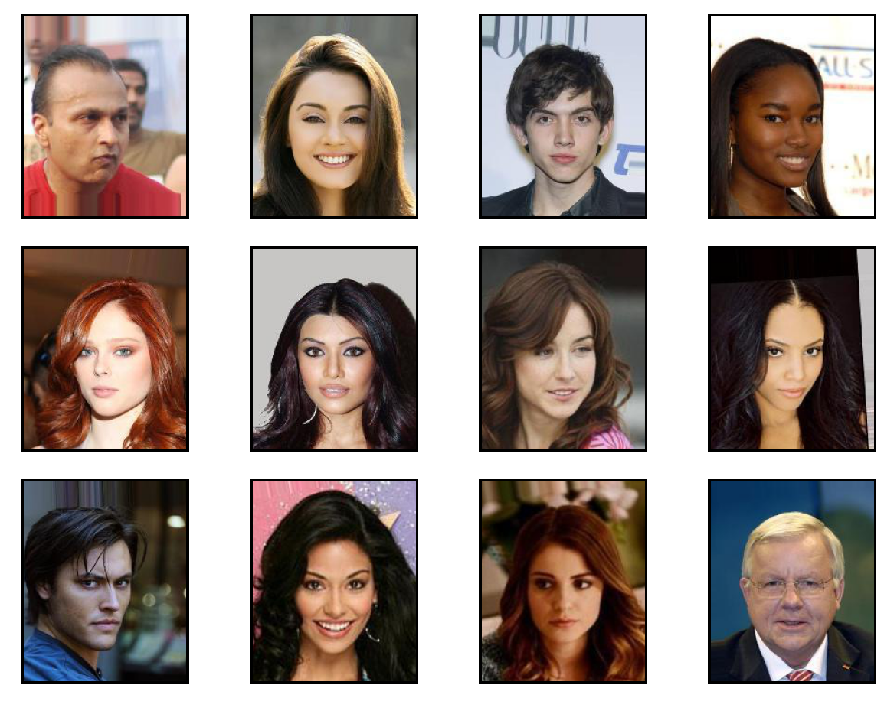
\includegraphics[width=0.8\textwidth]{chapters/Datasets/figures/CelebA.pdf}
    \fonte{From the author (2021)}
    \label{fig:dataset_celeba}
\end{figure}

\chapter{Datasets} \label{cha:datasets}
To understand the concepts explored in this document it is sometimes helpful to bring real world examples in order to represent the theoretical ideas in more familiar terms. This chapter will introduce the datasets relevant to this document, used for explaining the concepts, but mostly for performing the experiments that will be described in \autoref{cha:experiments}.

For any machine learning problem there is the desire to model something, some practical examples could be: how likely a person is to have a disease given a set of medical conditions; what type of animal an image represents; or what is the best move to make given a board position in chess. Whatever the underlying situation being modeled, it is necessary to have some data to build the model around.

This data can be obtained through self play (e.g. in Reinforcement Learning problems), but in the majority of cases it is given by a dataset. A dataset is simply a collection of samples from the situation being modeled, it does not contain all the possible values but, if sufficiently expansive, it should have enough samples to be a good representation of the distributions and particularities of the modeled situation. The goal of a dataset is to contain enough data, so that a machine learning algorithm trained on it can generalize well to data outside of it.

For neural networks a dataset is commonly divided into three groups: training, validation and test data. The training data is used in the learning process, it is what the network will see and will try to model, given this importance it is usually the largest chunk of a dataset. The validation data on the other hand is used to decide how to build the network and how to train the model, another way of saying this is that the training data is used to tune the network's parameters, while the validation data is used to tune the hyperparameters (see \autoref{sec:loss_&_gradient_descent}).

The validation process consists of training several models on the usually smaller validation data and seeing which set of hyperparameters produced the better results. One might wonder why would there be a need for this data and why not just use the training data instead? The main benefit of using a different set for validation is that validating on the training data has the risk of finding a set of hyperparameters that is particularly good on this data but that does not generalize well, using a separate validation data is a way to not overfit the hyperparameters to the training data and achieve better generalization.

The last chunk of a dataset, the test data, is used to validate the quality of the model and it's hability to generalize. This data should never be used to update either the parameters or hyperparameters, it should instead only be used as an evaluation tool, a way to estimate how well the model will perform on unseen data.

The next sections will explore the datasets relevant to the experiments made for this document. It is usual for datasets to already come separated into train and test data (the validation data is usually taken from a subset of the training data only if needed). This division will be mentioned for the described datasets, but it is relevant to note that any other divisions could also be obtained by combining and redistributing the data differently.


\section{MNIST} \label{sec:mnist}
\glsreset{MNIST}
Introduced in 1998 by \textcite{mnist1998}, the \gls{MNIST} is one of the most popular datasets in the field of machine learning, it's simplicity has made it a perfect choice as an introduction to deep learning and classification problems \cite{NN&DL2015}, but also as a benchmark for new techniques in serious research \textbf{--} some examples include \cite{dropout2012}, \cite{gans2014}, \cite{conditionalGAN2014} and \cite{adam2017}.

This dataset consists of 70,000 (60,000 training and 10,000 test) gray-scale images of handwritten digits, all images are of size $28{\times}28$ pixels and are labeled with the corresponding digit. The pixel values are inverted, this means that the strength of the strokes are represented with white pixels (values close to 255) against a black background (pixel value 0), this is however just how the data is represented numerically, for visualization purposes it is better to invert the colors as seen on \autoref{fig:dataset_mnist} \textbf{--} This figure shows some samples from this dataset along with the corresponding label.
\begin{figure}[hbt]
    \centering
    \caption{Labeled samples from the MNIST dataset}
    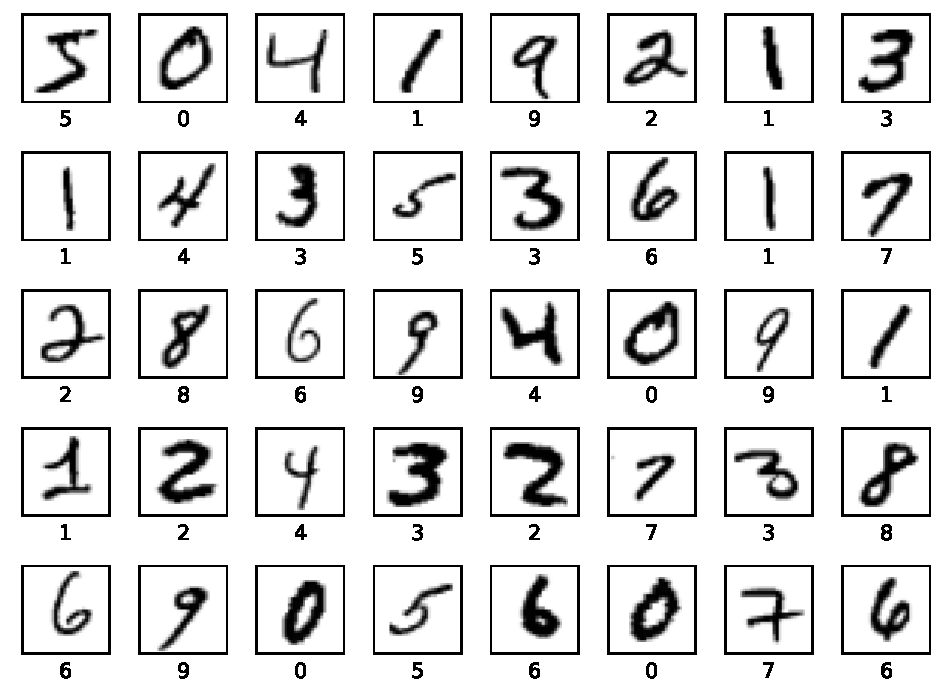
\includegraphics[width=0.6\textwidth]{chapters/Datasets/figures/MNIST.pdf}
    \fonte{From the author (2021)}
    \label{fig:dataset_mnist}
\end{figure}


\section{Fashion MNIST} \label{sec:fashion_mnist}
The simplicity of the \gls{MNIST} dataset makes it a very natural choice for benchmarking a Neural Network, however the data that it represents is also very simplistic \textbf{--} \textcite{mnistSOTA2013} were able to achieve a classification error lower than 0.3\% on the test set. The fact that \gls{MNIST} can be too easy has raised some questions about the usefulness of this dataset in benchmarking methods that scale to more complex tasks.

In response to these questions \textcite{fashionMNIST2017} proposed the Fashion MNIST dataset, arguing that \gls{MNIST} is too easy and cannot represent modern computer vision problems. Their goal was to replace \gls{MNIST} with a more robust dataset, without losing the simplicity of use that made the original so popular in the first place.

The Fashion MNIST dataset has all the same properties of \gls{MNIST}, it consists of 70,000 (60,000 training and 10,000 testing) $28{\times}28$ gray-scale images labelled from 0 to 9. The images however do not represent handwritten digits, they are instead preprocessed pictures of clothing items from the Zalando fashion company \cite{fashionMNIST2017}, the labels directly map to the type of clothing represented. Just like in \gls{MNIST}, the pixel values for the images are also inverted, the authors have made an effort to make the change of datasets as simple as just changing the link to get the files.

\autoref{fig:dataset_fashion_mnist} shows some labeled samples from this dataset, the pixel values are inverted for better visualization.
\begin{figure}[hbt]
    \centering
    \caption{Labeled samples from the Fashion MNIST dataset}
    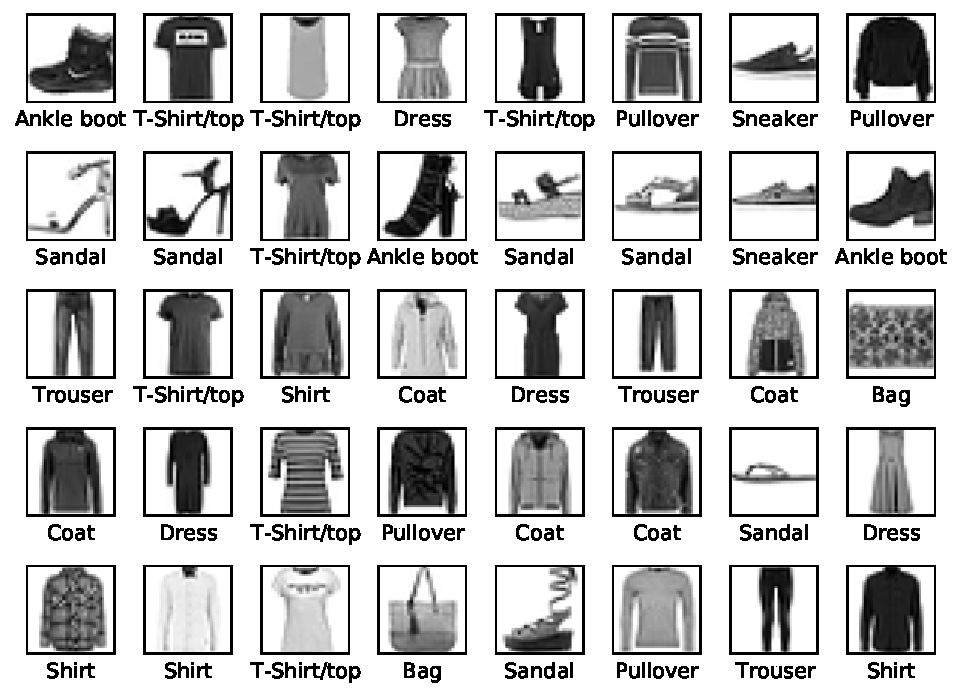
\includegraphics[width=0.7\textwidth]{chapters/Datasets/figures/Fashion_MNIST.pdf}
    \fonte{From the author (2021)}
    \label{fig:dataset_fashion_mnist}
\end{figure}


\section{CIFAR-10} \label{sec:cifar}
The \gls{CIFAR} datasets, \gls{CIFAR}-10 and \gls{CIFAR}-100, are two different subsets of the much larger 80 Million Tiny Images dataset, both are made of 60,000 (50,000 training and 10,000 testing) colored natural images of size $32{\times}32$ that were labeled by paid students to fit in a set of classes.

The images from \gls{CIFAR}-10 are divided into 10 classes with 6,000 images each, while \gls{CIFAR}-100 has 100 classes with 600 images each \cite{cifar2009}. For this document, only the \gls{CIFAR}-10 dataset was chosen for the experiments.

The \gls{CIFAR} datasets are another very popular choice for benchmarking neural networks, but given that they consist of colored images with increased resolution and more complex classes they offer considerably more challenge when compared to the \gls{MNIST} dataset. \autoref{fig:dataset_cifar10} shows examples of labeled samples taken from the \gls{CIFAR}-10 dataset.
\begin{figure}[hbt]
    \centering
    \caption{Labeled samples from CIFAR10 dataset}
    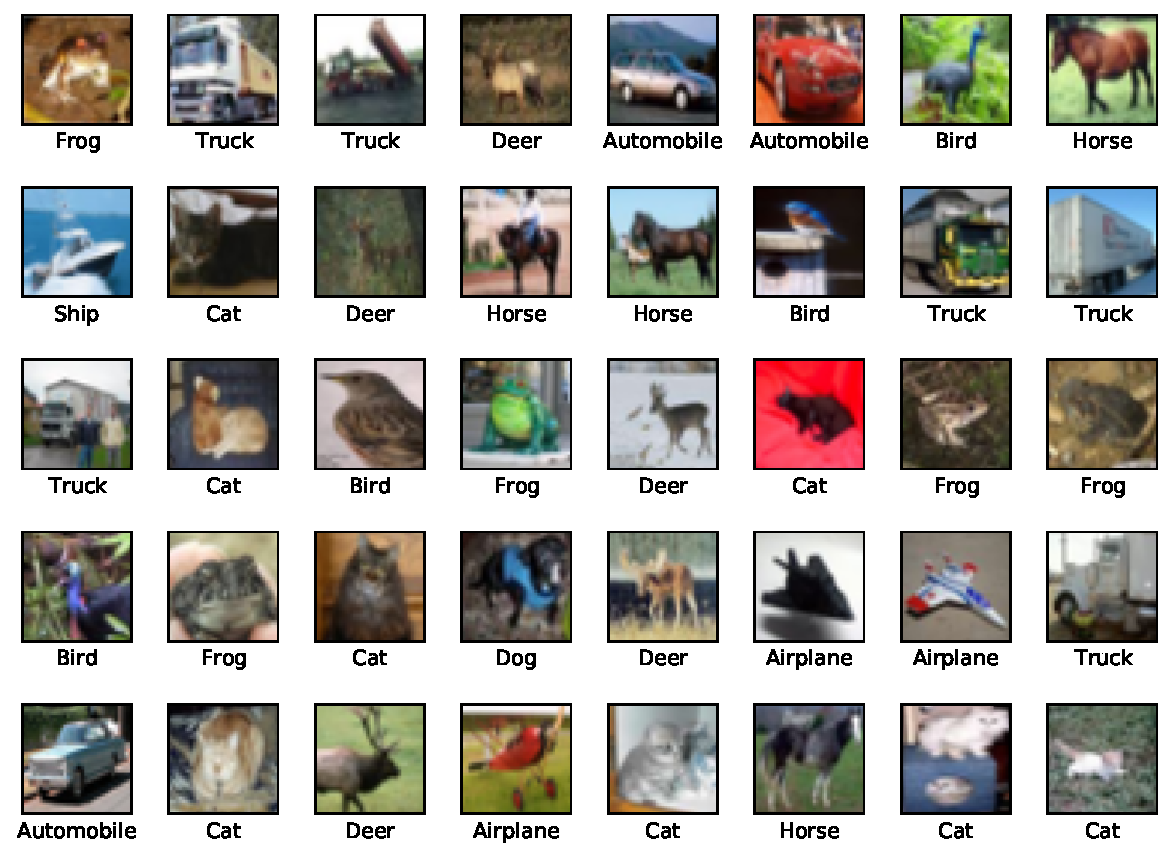
\includegraphics[width=0.7\textwidth]{chapters/Datasets/figures/CIFAR10.pdf}
    \fonte{From the author (2021)}
    \label{fig:dataset_cifar10}
\end{figure}



\section{Flowers} \label{sec:flowers}
The flowers dataset consists of $8,189$ high resolution images of 102 different categories of flowers, each category has from 40 to 250 different images \cite{flowers2008}. Samples from this dataset can be seen on \autoref{fig:dataset_flowers}

\begin{figure} [hbt]
    \centering
    \caption{Samples from the Flowers dataset}
    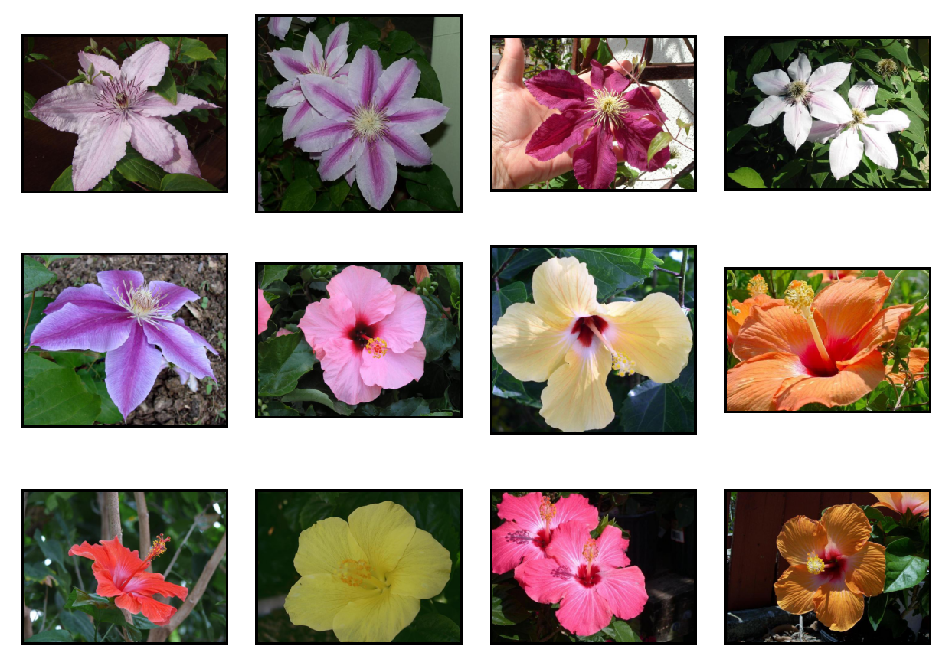
\includegraphics[width=0.8\textwidth]{chapters/Datasets/figures/Flowers.pdf}
    \fonte{From the author (2021)}
    \label{fig:dataset_flowers}
\end{figure}

\section{CelebA} \label{sec:celebA}
This is the largest dataset used in this document in terms of number of elements, it consists of $202,599$ pictures of faces of celebrities, all rescaled to size $178\times218$. All images are heavily annotated, having $40$ binary features (e.g. blonde hair, eyeglasses, wearing hat, young) and the positions of eyes, nose and mouth all labeled \cite{celebA2015}. However, for the purposes of this document the annotations will not be relevant. \autoref{fig:dataset_celeba} shows examples of pictures in this dataset.
\begin{figure}
    \centering
    \caption{Samples from the CelebA dataset}
    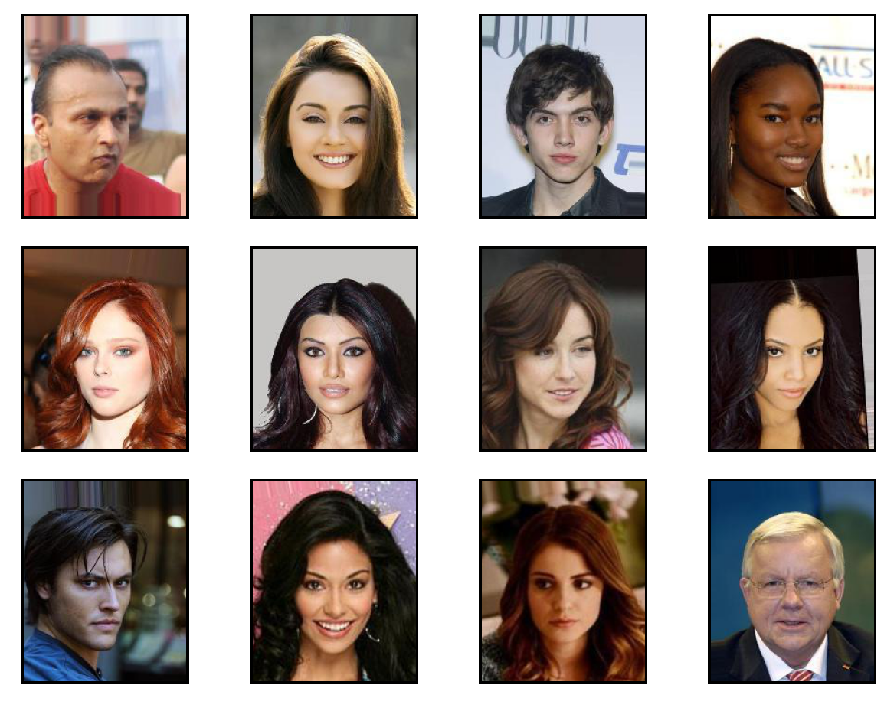
\includegraphics[width=0.8\textwidth]{chapters/Datasets/figures/CelebA.pdf}
    \fonte{From the author (2021)}
    \label{fig:dataset_celeba}
\end{figure}


% ----------------------------------------------------------


% -- ELEMENTOS PÓS-TEXTUAIS  -------------------------------
\postextual

% Referências
\begingroup
    \SingleSpacing\printbibliography[title=REFERÊNCIAS]
\endgroup

%Apêndices
\begin{apendicesenv}
	\chapter{Specifications of the Machine} \label{apd:machine_specs}
The main components of the machine which ran the experiments consist of:
\begin{itemize}
    \item \textbf{Processor} AMD FX(tm)-6100 Six-Core 3.3 GHz
    \item \textbf{RAM} 4.0 GB
    \item \textbf{Video Card} NVIDIA GeForce GTX 1050, 2.0GB Dedicated Memory, 4.0GB Total Memory
    \item \textbf{Tensorflow} version 2.3.0
\end{itemize}
\end{apendicesenv}

% Anexos
% \begin{anexosenv}
% 	\input{aftertext/anexo_a}
% \end{anexosenv}

% ----------------------------------------------------------


\end{document}
